\documentclass[nochap,palatino,shortheader]{apuntes}

\title{Organización de Empresas Tecnológicas}
\author{Guillermo Julián\and Pedro Valero \and Victor de Juan}
\date{2016}

% Paquetes adicionales
\usepackage{fancysprefs}
\usepackage{booktabs}
\usepackage{multirow}
\usepackage{textcomp}
\usepackage{tikztools}
\usepackage{changepage}
%\usepackage{soul}
\usepackage{soulutf8}


\newcommand{\study}[1]{#1}
\newcommand{\substudy}[1]{#1}
\setulcolor{Orange}


\begin{document}
\pagestyle{plain}

\begin{abstract}
Este documento recoge todos los contenidos vistos en la asignatura ``Organización de Empresas Tecnoloógicas'', impartida en la Escuela Politécnica Superior de la Universidad Autónoma de Madrid por el profesor Fernando Maestre Miranda.

Para la elaboración de estos apuntes se han tomado como base las transparencias proporcionadas por el profesor y usadas para presentar la asignatura en las clases teóricas, completadas con los principales conceptos explicados en estas clases.

Salvo que se indique lo contrario, las imágenes presentadas en este documento proceden son extractos de las transparencias presentes en la \href{http://maestremiranda.com}{web del profesor}.
\end{abstract}

\maketitle

\tableofcontents
\newpage
\section{Empresa}

\subsection{La Empresa y el Empresario}

Antes de comenzar a ver esta sección, conviene darnos cuenta de lo poco que sabemos al respecto. En nuestro día a día creemos saber qué es una empresa (y consecuentemente, qué es un empresario) pero hagamos el ejercicio de intentar definirlo de manera formal.

Una vez creemos que ``sabemos'' de antemano cuál es esta definición, parémonos a pensar en las siguientes preguntas:

\begin{itemize}
\item ¿Es un taxista un autónomo?
\item ¿Y un fontanero?
\item ¿Un kiosko de la calle es una empresa?
\item ¿Y un puesto de chucherías?
\end{itemize}

Si el lector se para a hacer este ejercicio verá que le surgen un montón de dudas al respecto, muchas de ellas en lo referente a los límites que separan a un \textbf{autónomo} de un \textbf{empresario}.

A fin de aclarar estos conceptos veamos algunas definiciones pseudo-formales\footnote{A lo largo de este documento emplearemos definiciones de este tipo a fin de que el lector comprenda los conceptos sin necesidad de aprender una jerga complicada y enrevesada.}.

\begin{defn}[Autónomo]
En España, un \textbf{trabajador autónomo} (no confundir con un empresario individual), es la persona física que realiza de forma habitual, personal y directa una actividad económica a título lucrativo sin sujeción a contrato de trabajo.
\end{defn}

\begin{defn}[Franquicia]
Práctica de utilizar el modelo de negocio de otra persona o empresa.
\end{defn}

\begin{defn}[Grupo empresarial]
Es el conglomerado de empresas que dependen todas de una misma empresa matriz que tiene suficiente participación económica en sus capitales como para tomar decisiones
\end{defn}

\begin{defn}[Empresa]
Una \textbf{empresa} es una \textbf{unidad económico-social} integrada por elementos humanos, materiales y técnicos, que tiene el objetivo de obtener utilidades a través de su participación en el mercado de bienes y servicios. Para esto hace uno de los \textbf{factores productivos} (trabajo, tierra y capital).

El control de la empresa lo ejercen los propietarios, que se organizan en un consejo de administración. En el día a día, los directivos son los que dirigen la empresa.

\end{defn}
\newpage
Las empresas pueden constituirse, principalmente, de dos formas:
\begin{enumerate}
\item Como \concept{Sociedad\IS Anónima (SA)}. Se trata de una sociedad eminentemente capitalista, es decir, en ella se valora más el capital que cada socio aporta que las características personales de los mismos y por eso \textbf{es la sociedad adecuada para desarrollas la actividades en las que se prevea la participación de un gran número de socios, así como una mayor movilización de capital}.

La legislación española establece que las sociedades anónimas deben tener, como mínimo, un capital de 60.000 euros del que, al menos, un 25\% deberá estar desembolsado en el momento de firmar la escritura pública.

Las sociedades anónimas tienen acciones (no participaciones) al portador, que se pueden vender y comprar libremente (por eso sólo las SA cotizan en bolsa).


\item Como \concept{Sociedad\IS Limitada (SL)} . Sin dejar de ser una sociedad capitalista, participa de los caracteres propios de las sociedades personalistas o de los contratos celebrados ``intuitu personae'', es decir, aquellas en las que, aún siendo importante el capital que cada socio aporta, también se da importancia a las cualidades personales de los socios que la integran.

La legislación española establece que las sociedades anónimas deben tener un capial mínimo de 3000 euros, que puede estar o no totalmente desembolsado\footnote{Ingresado en la cuenta de la sociedad} en el momento de firmar la escritura pública.

Los socios no pueden vender libremente sus participaciones (los estatutos ponen las normas bajo las cuales pueden realizarse estas ventas), salvo a familiares directos.
\end{enumerate}

Ambas sociedades están reguladas por el \href{https://www.boe.es/buscar/act.php?id=BOE-A-2010-10544}{RD 1/2010 de 2 de julio}. Aunque puede pensarse que la distinción entre estos tipos de sociedades depende del número de integrantes, esto no es así. Ambas tienen también versiones unipersonales.

La siguiente imagen nos da una representación esquematizada de definición/organización de una empresa.

\begin{center}
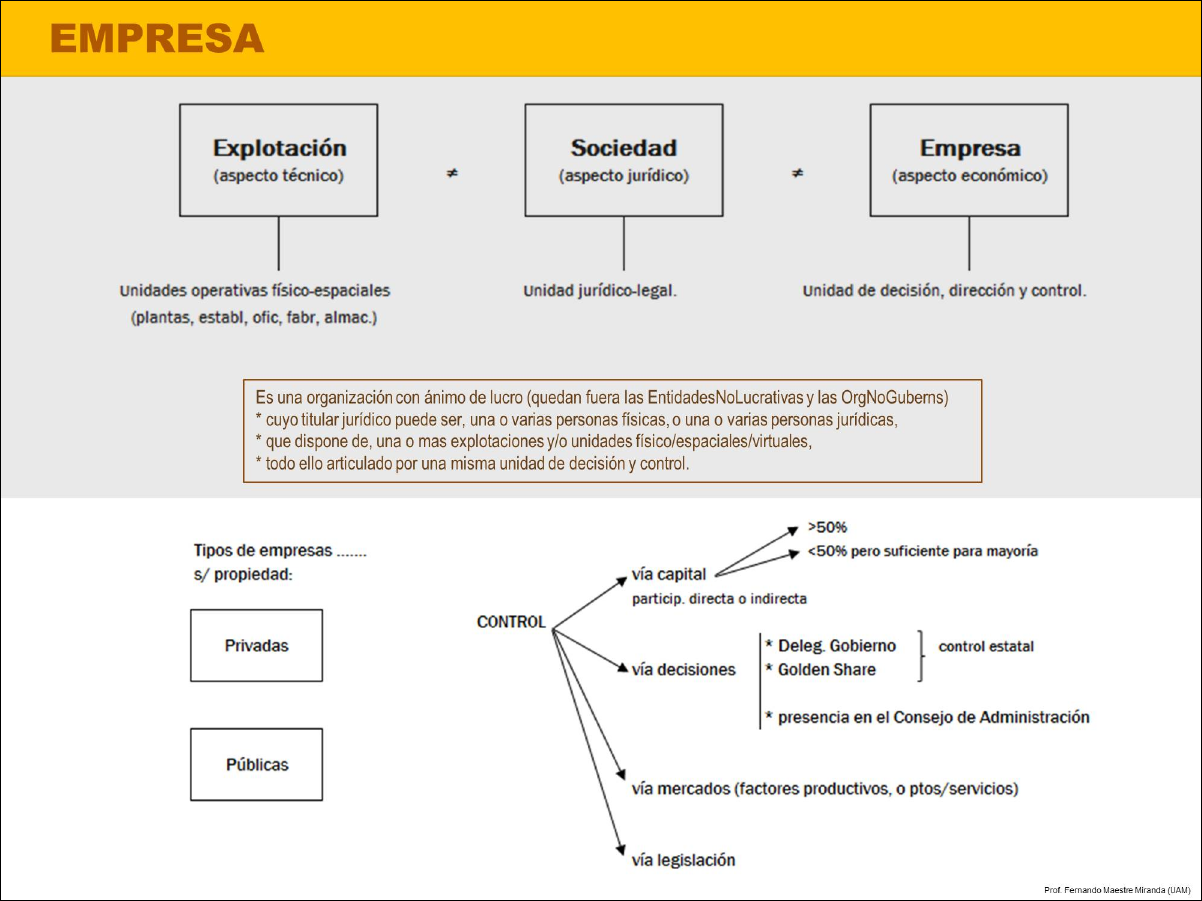
\includegraphics[width=0.7\textwidth]{img/empresa.png}
\label{fig:EstructuraEmpresa}
\end{center}

Las empresas pagan impuestos a través del Impuesto de Sociedades y de la Seguridad Social. 

Si la empresa \study{quiebra, sólo se responde con el patrimonio de la empresa} y no con el de los socios (al contrario de lo que ocurre si una persona es un \study{autónomo, que responde de las deudas con todo su patrimonio).}

En cualquiera de los dos casos, es importante ver la relación laboral que tienen los directivos y administradores con la empresa. Los altos directivos\footnote{Los que ejercitan poderes que corresponden a los titulares de la empresa con autonomía y plena responsabilidad (limitadas únicamente por los órganos de gobierno de la empresa).} tienen una relación de carácter especial con la empresa, no regulada por el \href{https://www.boe.es/buscar/act.php?id=BOE-A-1995-7730&tn=1&vd=&p=20151024}{Estatuto de los trabajadores} sino por el \href{https://www.boe.es/diario_boe/txt.php?id=BOE-A-1985-17006}{Real Decreto 1382/1985}, aunque a efectos prácticos el contrato es un contrato laboral. Sin embargo, si los altos directivos realizan tareas de administración o gerencia en la empresa (por ejemplo, consejeros), ya no hay relación laboral sino mercantil, y por lo tanto el directivo en cuestión debe darse de alta en el régimen de autónomos.

La siguiente imagen representa, de modo esquemático, las diferencias entre \concept{directivos} y \textbf{accionistas}.

\begin{center}
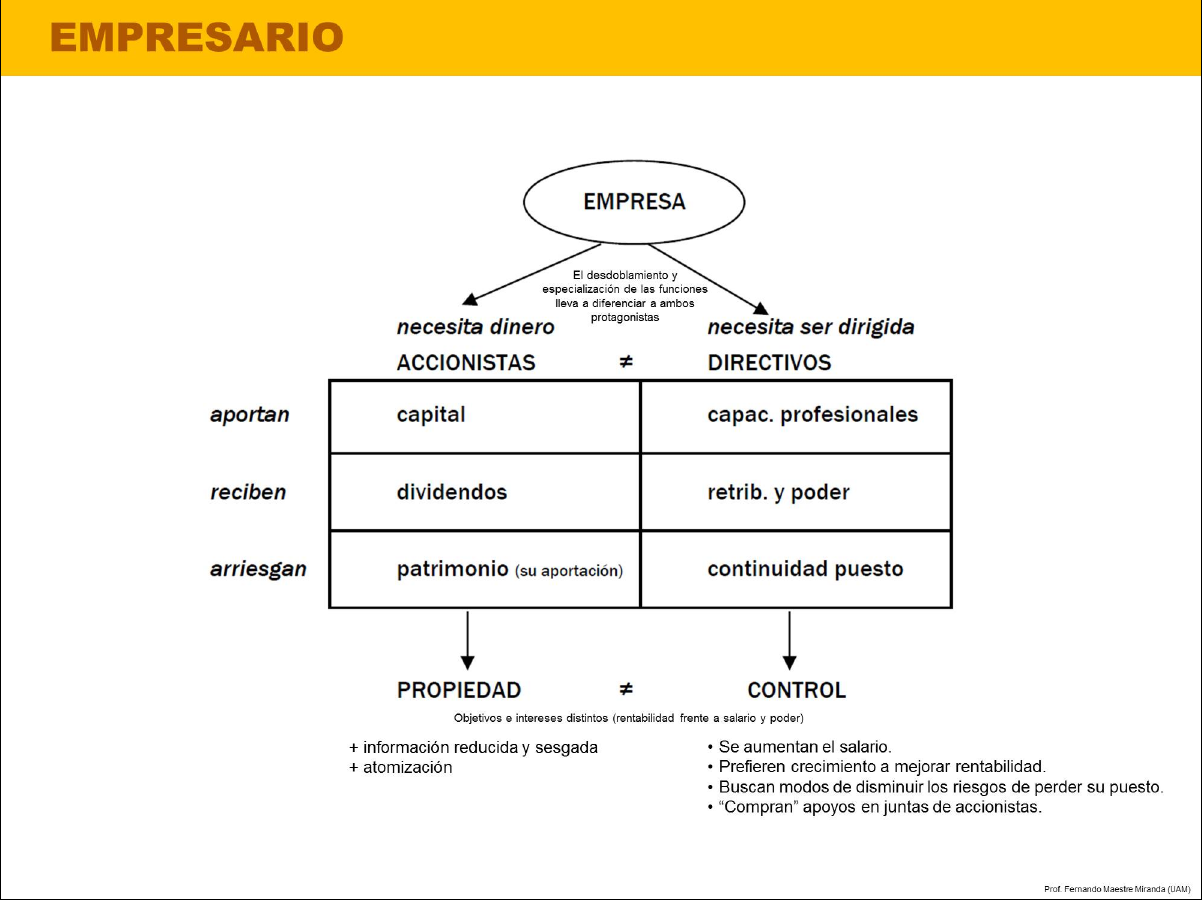
\includegraphics[width=0.7\textwidth]{img/empresario.png}
\label{fig:AccionistasVSDirectivos}
\end{center}

\subsection{Guía para la creación de una empresa (sociedad)}

Para crear una empresa, hay que seguir la burocracia correspondiente. En general, hay que seguir los siguientes pasos, sacados de la \href{http://www.creatuempresa.org/es-ES/PasoApaso/}{página del Ministerio de Industria}.

\begin{enumerate}
\item Ir al Registro Mercantil para acreditar que no hay otra sociedad con el mismo nombre que la que queremos constituir.
\item Ir a la AEAT\footnote{Agencia Estatal de Administración Tributaria, también llamada Agencia Tributaria o Hacienda.} a obtener un CIF provisional.
\item Ir al banco y desembolsar el capital social en una cuenta a nombre de la empresa (para esto necesitamos el CIF provisional).
\item Ir al notario para firmar la escritura de Constitución de la Sociedad. Hay que llevar los estatutos sociales, la acreditación del desembolso del capital social y los documentos de identidad de los socios.
\item Ir al Registro Mercantil provincial para inscribir la sociedad.
\item Ir al Ayuntamiento a pagar el impuesto sobre Actividades Económicas (IAE), aunque últimamente hay exenciones.
\end{enumerate}

El apéndice \ref{sec:CreacionEmpresa} muestra una versión esquematizada del proceso de creación de una empresa.

La \study{constitución de una empresa} conlleva la \study{obligación de declarar} ciertas acciones, como la modificación de estatutos sociales, aumentos y reducciones de capital, nombramiento y cese de administradores, aperturas y cierres de sucursales. También tendrá que presentar las cuentas según indique la legislación vigente (ver \fref{sec:Contabilidad}).

Los \study{administradores} de la empresa pueden ser \study{organizarse} de forma \study{\textbf{solidaria}}, lo que hace que todos ellos tengan poder de decisión sobre la empresa y su firma sea aceptada como representación de la entidad completa; o \study{\textbf{mancomunados}}, donde es necesaria la firma de todos a la hora de tomar cualquier decisión. % TODO: Algo de autónomos societarios.

Otra opción para constituir una empresa si no queremos morir ahogados en burocracia es usar el \href{http://www.creatuempresa.org/es-ES/PasoApaso/Paginas/etramitacion.aspx?cod=SRL&nombre=Sociedad%20de%20Responsabilidad%20Limitada&idioma=es-es}{sistema CIRCE}\footnote{Centro de Información y Red de Creación de Empresas}, que nos permite realizar todos los trámites teniendo que ir sólo a la notaría. Sólo tendremos que reservar el nombre, aportar el capital, cumplimentar el Documento Único Electrónico (podemos ir además a un centro PAE\footnote{Punto de atención al emprendedor.} a que nos ayuden) y después ir al notario a que nos haga el resto del trabajo. Además, se podrán realizar algunos trámites adicionales.

\subsubsection{Curiosidades de la vida real}
Lo que acabamos de ver muestra el procedimiento básico y sencillo para la creación de una empresa pero el resultado obtenido dista mucho de la realidad en la que viven las grandes empresas que todos conocemos.

A fin de evitar responsabilidades jurídicas y/o civiles, las empresas se constituyen en un complejo entramado. Puesto que el dueño de una sociedad puede ser una \textbf{Persona Jurídica}, nos acabamos encontrando con empresas que se unen en grupos de empresas cuyos dueños son otras empresas que, a su vez, se organizan en grupos de empresas...

%TODO completar con las transparencias de clase o con algo que tenga la gente el follon que se encuentra uno si trata de encontrar el mandamas de ZARA, por ejemplo.

Antes de ver más detalles acerca de estas ``telarañas'' que se constituyen en la vida real, veamos algunas definiciones más:

\begin{defn}[Levantamiento de velo]
Investigar quiénes son los socios de una empresa.

Esta actividad se lleva a cabo sólo de manera excepcional para averiguar quién está detras de una empresa. Es una tarea muy compleja por la difícil delimitación de las responsabilidades.
\end{defn}

\begin{defn}[Alzamiento de bienes]
Consiste en ocultar parte (o el total) del patrimonio para que el acreedor no pueda cobrarse su deuda.

El alzamiento de vienes es una manera de declarar insolvencia, pero es un delito (no todas las formas de insolvencia son delitos \textbf{pero las de este tipo sí}).
\end{defn}

Además de esto, las empresas suelen mantener de manera simultánea dos contabilidades, sin que esto implique incurrir en ningún tipo de delito.

Una de estas contabilidades organiza los pagos, cobros, inversiones, amortizaciones, etc de la empresa (conceptos que veremos más adelante) de forma que se obtenga el mayor beneficio fiscal posible, siempre dentro de la legalidad.

El problema de esta contabilidad es que dificulta tener una visión real de la situación de la empresa, para lo que se mantiene una segunda contabilidad. Mas adelante estudaremos los conceptos necesario para poder comprender estas diferentes contabilidades.


\subsection{Patentes}

La idea de la patente es dar al inventor de un invento, valga la redundancia, el \textbf{derecho exclusivo a explotarlo}. Por ejemplo, inventas firulillos voladores y, si los patentas, nadie más podrá fabricarlos salvo que les des permiso (normalmente, a cambio de una cuota o \textit{royalty}). La principal ventaja es que se evitan los plagios y se protege a los inventores del abuso por parte de empresas con más recursos.

Aunque el ejemplo que se acaba de comentar puede parecer una tontería lo cierto es que no lo es. Algunos ejemplos de ideas patentadas son el concepto del \textit{doble click} o el uso de \textit{rectángulos con esquinas redondeadas}.

No obstante, no siempre resulta interesante patentar un invento pues esto implica poner todos los detalles a disposición pública. Nadie podrá copiarlos, pues estarán obligados a pagar por ley al dueño de la patente, pero puede servir de inspiración a otros que acaben superando tu idea.

Por ejemplo, Apple no patenta sus productos y se centra en el \textbf{secreto industrial} para proteger sus inventos.

Lo malo es que las patentes también se pueden utilizar como arma arrojadiza. Se pueden patentar cosas extremadamente genéricas y utilizarlas para demandar a otras empresas. No hace falta mencionar casos como los de la guerra de patentes entre tecnológicas.

En España, la entidad encargada de gestionar las patentes es la Oficina Española de Patentes y Marcas.

\subsection{Organización y funciones empresariales}

Hay que recalcar que no hay una estructura ``estándar'' para organizar una empresa. No obstante, algunos de los modelos más empleados son:
%TODO que julian haga el dibujito.
% El dibujito de qué?

Vamos a centarnos en el análisis del caso más ``clásico'', la estructura jerárquica. Esta estructura queda representada con más detalle en el siguiente esquema:

\begin{center}
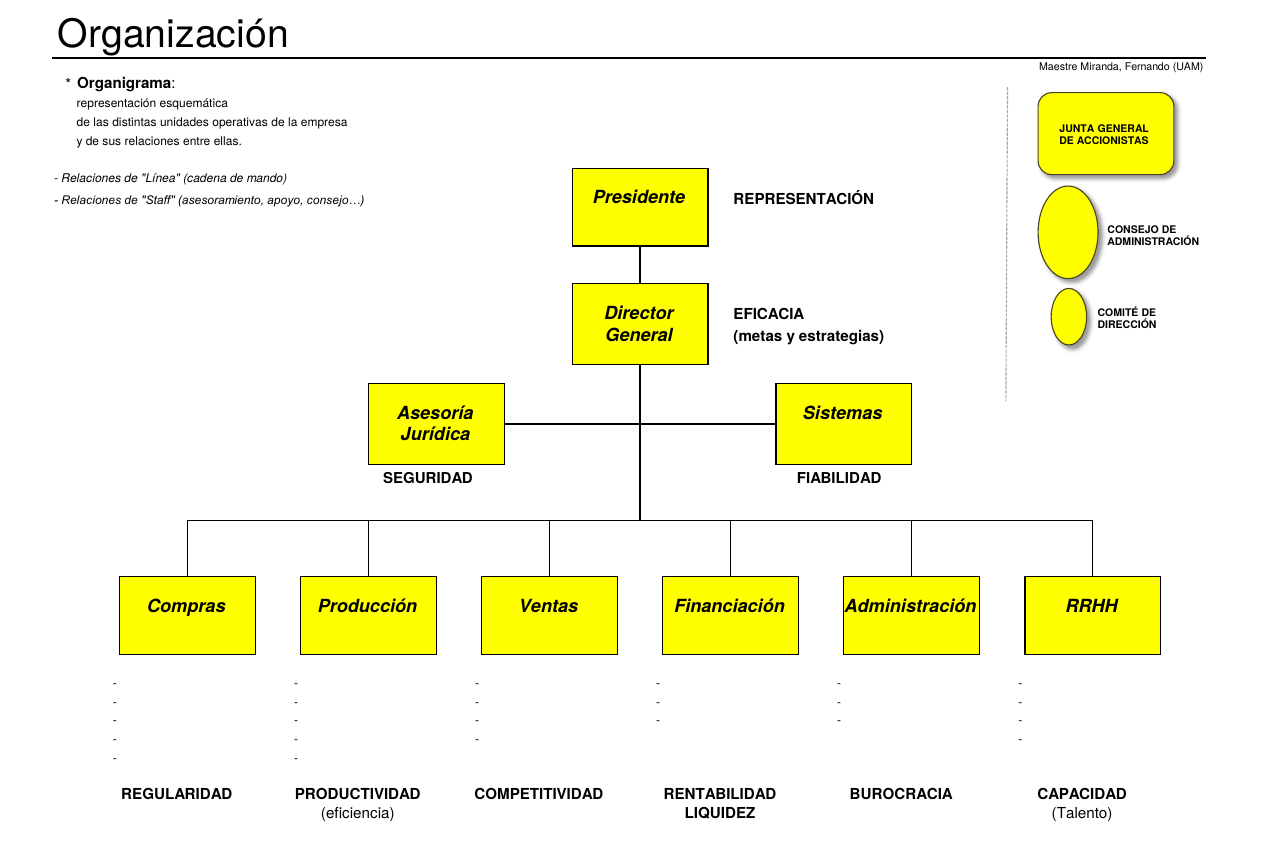
\includegraphics[width=0.9\textwidth]{img/organizacionEmpresa.png}
\label{fig:organizacionEmpresa}
\end{center}


Habitualmente tendremos al presidente, que será el que represente a la empresa y además el que establezca las estrategias generales. En un nivel similar, tendríamos la junta general de accionistas y su versión reducida, el consejo de administración. También tendríamos el Comité de dirección, con las mismas metas de estrategia general.

Ya entrando en el día a día, tendríamos al \concept{Director\IS general} o ejecutivo de la empresa, el ejecutivo con más poder dentro de la empresa. En empresas pequeñas, el presidente y director general suelen ser la misma persona.

Dentro de la empresa, se pueden organizar distintos departamentos (ver \fref{tab:Organizacion}) para distribuir la actividad, dependientes del director general.

\begin{table}[hbtp]
\centering
\begin{tabular}{l|p{5cm}|p{5cm}}
\textbf{Departamento} & \textbf{Descripción} & \textbf{Funciones} \\ \toprule
Compras & Abastecen a la empresa con los recursos necesarios para funcionar, como \textit{stock} o equipamiento de fabricación. & Abastecimiento, Calidad del género recibido, Inversión equipamiento, Negocación con proveedores \\ \midrule

Producción & Obvio. Buscan aumentar productividad y eficiciencia. & Gestión de stock, Control de calidad de producto, I+D \\ \midrule

Ventas & Venden el producto, buscan ser competitivos frente a otros. & Investigación de mercados, Postventa, Precio, Promoción \\ \midrule

Financiación & Manejan el dinero, se aseguran de que haya suficiente para funcionar y que los gastos no sean excesivos. & Captación de recursos financieros, Contabilidad, Evaluación de inversiones \\ \midrule

Administración & Burócratas. & Facturación, Tesorería, Nóminas \\ \midrule

Recursos Humanos & Gestionan empleados de la empresa. & Formación\\ \midrule \midrule
Asesoría jurídica & Dan seguridad jurídica al funcionamiento de la empresa & \\ \midrule
Sistemas & Se encargan de que los sistemas informáticos funcionen bien y sin problemas. & \\
\end{tabular}
\caption{Departamentos de una empresa y posibles atribuciones. Las funciones de la columna de la derecha salen de \href{http://maestremiranda.com/techdir/wp-content/uploads/2015/10/Organizacion2.pdf}{FMM}. Los dos últimos departamentos no son directamente subordinados del director general, sino más bien asesores.}
\label{tab:Organizacion}
\end{table}

\subsection{Ciclo de explotación}

El ciclo de explotación se la secuencia de pasos por los que se mueve la empresa al comprar materiales, transformarlos en un producto, venderlo y cobrarlo. De esto, lo interesante la \study{optimización de stock}. 
Sólo dos conceptos previos que aparecen en los apuntes: la \concept{Rotación\IS de stock}, que se refiere a la cantidad de entradas de \textit{stock} entre el \textit{stock} medio, y la \study{duración}, que se refiere a cuántos días nos dura cada rotación. Fácil y sencillo.

El apéndice \ref{sec:cicloExplotacion} ilustra el concepto de \textbf{ciclo de explotación}.

\subsubsection{Optimización de stock}

El problema de la optimización de stock viene por un conflicto a la hora de mantener un almacén de productos, como plastafurbos\footnote{\href{http://mundowdg.com/blog/2009/04/16/adioshola/}{En honor a Wardog, blog que todo informático debería leer}, plastafurbo será mi palabra comodín cuando hable de productos que se puedan vender. A efectos prácticos pues, plastafurbo = producto.} a vender. 
Por un lado, queremos mantener un almacén lo más pequeño posible: no queremos que nuestros productos se queden obsoletos o caduquen y queremos gastar el menor dinero posible en almacenarlos. 
Además, es mejor tener nuestro dinero en billetes que en plastafurbos, ya que nos dará más agilidad cuando necesitemos invertir el dinero en otras cosas.

Por otro, si nuestro almacén es pequeño podemos encontrarnos con que no podemos vender plastafurbos a nuestros clientes, cosa que todos podemos imaginar que es increíblemente mala (esto se llama \concept{Rotura\IS de Stock}). 
Si además hacemos muchos pedidos pequeños para compensar, tendremos un coste de compra mayor (normalmente, si compramos muchas cosas hay descuento por volumen). Aun así, eso no nos libraría de roturas de stock si nuestra demanda fluctúa mucho.

\begin{figure}[hbtp]
\centering
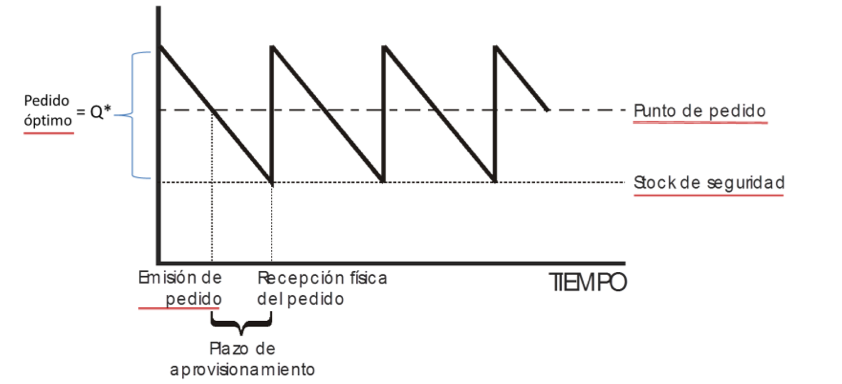
\includegraphics[width=0.8\textwidth]{img/ControlStock.png}
\caption{Ejemplo de pedidos óptimos, vía FMM.}
\label{fig:StockDeterminista}
\end{figure}

La optimización de stock es un problema matemático muy interesante de estudiar en profundidad\footnote{Más que nada porque son matemáticas.}. Se trata de modelar la demanda y el comportamiento de los proveedores para encontrar el momento en el que hacer el pedido y la cantidad para minimizar costes y evitar roturas de stock. 

Los \study{modelos} usados pueden ser \study{deterministas}: por ejemplo, miramos las ventas por día y vemos a qué nivel de stock debemos de hacer un pedido contando con lo que tarda el proveedor, de tal forma que nos llegue el pedido justo al llegar al margen mínimo de seguridad (ver \fref{fig:StockDeterminista}).

El siguiente paso son los \study{modelos estocásticos}\footnote{Es una forma bonita de hablar de procesos aleatorios y que además parezca que sabes de qué estás hablando.}, donde tenemos en cuenta distribuciones de probabilidad para ciertas variables. 
Así, la demanda no es fija sino que podría venir dada por una distribución normal, y podríamos tener en cuenta la distribución del tiempo que tardan los distribuidores en traernos el pedido para así tener más claras las posibilidades de rotura de stock y poder seguir funcionando teniendo en cuenta fuentes de volatilidad.

Merece una mención el modelo \concept{Just In Time}, llevado a cabo por Toyota, por ejemplo. En lugar de mantener inventario, confían en los distribuidores para que les den los componentes en el momento en el que los necesitan, y así no tienen almacén.

\subsubsection{Valoración de stock}

La valoración del stock es otro problema, aunque menos interesante que el anterior. Cuando vendemos un plastafurbo, tenemos que ver cuánto hemos ganado con él. Y para eso necesitamos saber cuánto nos ha costado. El coste depende del coste de las materias primas y del coste de producción, costes que pueden variar a lo largo del tiempo. Así, si tenemos un almacén de \textit{stock}, cada plastafurbo tendrá un precio distinto. ¿Cuáles vendemos primero?\footnote{O, más concretamente, qué precio les ponemos. Si vendemos el plastafurbo al coste de las primeras fabricaciones, puede ser perfectamente un plastafurbo que justo acabamos de fabricar. Todo esto es sólo a nivel contable } El coste que atribuyamos a esas ventas, afectará a nuestras cuentas de beneficios (y por lo tanto a los impuestos que pagamos) pero también a la valoración de la empresa y a la fiabilidad de nuestros estados financieros.


\begin{table}[hbtp]
\centering
\begin{tabular}{l|c|c|c}
 & \textbf{FIFO} & \textbf{LIFO} & \textbf{Media} \\ \toprule
Stock plastafurbos antiguos & \multicolumn{3}{|c}{10} \\ \midrule
Coste unidad (CU) plastafurbo antiguo & \multicolumn{3}{|c}{10} \\ \midrule
Stock plastafurbos nuevos & \multicolumn{3}{|c}{10} \\ \midrule
CU plastafurbo nuevo & \multicolumn{3}{|c}{20} \\ \midrule
Ingresos por venta de 15 plastafurbos & \multicolumn{3}{|c}{400} \\ \midrule \midrule
CU de los 10 primeros plastafurbos & 10 & 20 & 15 \\ \midrule
CU de los 5 últimos plastafurbos & 20 & 10 & 15 \\ \midrule
Coste total de los 15 plastafurbos & 200 & 250 & 225 \\ \midrule
\textbf{Beneficios} & \textbf{200} & \textbf{150} & \textbf{175} \\ \midrule \midrule
CU de stock restante & 20 & 10 & 15 \\ \midrule
\textbf{Valoración stock restante} (5 plastafurbos) & \textbf{100} & \textbf{50} & \textbf{75} \\ \bottomrule
\end{tabular}
\caption{Ejemplo de los tres métodos de valoración de stock}
\label{tab:ValoracionStock}
\end{table}

Hay tres métodos para valorar el stock (ver \fref{tab:ValoracionStock} para un ejemplo combinado), y en todos los casos suponemos entorno inflacionario (el precio de todo va aumentando a lo largo del tiempo).

\paragraph{FIFO} Los primeros objetos que vendemos son los primeros que fabricamos o compramos. Así, el coste de inventario se acerca más al coste de las últimas unidades que entraron.

\paragraph{LIFO} Marcamos como vendidos los productos que más tarde hemos fabricado. La cuenta de beneficios disminuye, al igual que lo hace la valoración del stock. No tiene sentido usar este método a nivel físico: si de verdad vendemos los últimos productos fabricados y nos dejamos los más viejos, acabaremos con un almacén de plastafurbos obsoletos que nadie querrá comprar. Así, este método sólo se usa a la hora de valorar el stock, y al disminuir la cuenta de beneficios permite ahorrarnos impuestos. De hecho, esta es una de las razones por las que está prohibido en muchos países.

\paragraph{\study{Media o media ponderada}} La media o media ponderada nos dará un coste a medio camino entre el de FIFO y LIFO, de tal forma que tenemos la ventaja de pagar menos impuestos que tiene LIFO pero sin falsear del todo la valoración de stock.

\subsection{Inversión y bolsa}

La inversión en bolsa parte de un hecho fundamental, que es que las empresas tienen propietarios, en plural, y cada uno de ellos tendrá un porcentaje de propiedad. Normalmente, el porcentaje de propiedad se divide en unidades llamadas \concept[Acción]{acciones} o participaciones.

Esa propiedad puede dar lugar a diversos derechos, como por ejemplo el de recibir una parte de los beneficios de la empresa (\concept{Dividendo}) o a poder participar en la toma de decisiones de la empresa a través del \concept{Consejo\IS de accionistas}.

Monetariamente, esas participaciones tienen un valor económico, un valor que será proporcional a la valoración de la empresa. Además, esas participaciones se pueden vender y comprar. La bolsa es el mercado donde las participaciones o acciones de empresas se venden y se compran.

Como en cualquier acción de compra y venta, el precio fluctúa por la ley de la oferta y la demanda, y esas fluctuaciones de precio permiten ganar dinero (y, por supuesto, perderlo) en la bolsa a través de operaciones.

Una nota: se pueden hacer \concept{Split} y \concept{Contrasplit} cuando se quieren agrupar o dividir acciones. Por ejemplo, un contrasplit sirve cuando las acciones cotizan a muy bajo valor: se agrupan varias y se convierten en una única acción con más valor, valor que probablemente bajará luego porque ahora se podrá dividir más (con las acciones antiguas, el precio mínimo estaría a 1 céntimo por acción, que igual es muy alto).

Una clara ventaja de la bolsa es que permite que gente con poco capital se convierta en ``dueño'' de una gran empresa multinacional, lo que le da derecho a beneficiarse del buen avance de dicha empresa. Si una nueva empresa tecnológica aparece en el mercado y vende acciones, estas se comprarán a un precio muy bajo por ser una empresa nueva, con lo que casi todo el mundo tendrá la posibilidad de participar activamente de este proyecto.

Con la compra de esas acciones la empresa obtiene financiación, que le permite trabajar y extenderse y, a la hora de obtener beneficios, estos son repartidos entre todos los accionistas en lugar de quedarse en manos de los creadores.

Por tanto, la bolsa permite, a priori, que muchas personas contribuyan en el desarrollo de una empresa aportando el capital necesario al inicio y obteniendo beneficios proporcionales cuando la empresa triunfe.

La gran pega que tiene la bolsa es el concepto de la especulación. Una vez se han vendido las acciones por primera vez y la empresa ha obtenido la financiación buscada, estas acciones no se quedan en manos de sus dueños (a veces si que lo hacen pero no es lo habitual) sino que, por lo general, son constantemente vendidas y compradas en el mercado.

Esto da lugar a que el precio de las acciones acabe siendo muy variable y funcione por ciclos lo que puede provocar que aún creciendo la empresa, alquien que haya comprado acciones pierda dinero.


\subsubsection{Operaciones en bolsa}

La operación más sencilla que uno puede hacer en bolsa es comprar una acción, esperar a que su valor suba porque más gente quiera comprar participaciones de la empresa (por ejemplo, si esa empresa va bien y los inversores esperan que siga así) y venderla para recoger los beneficios. Ahora bien, las cosas pueden complicarse un poco más, y de hecho la terminología cambia. A partir de ahora, consideraremos una \concept{Posición} como una inversión abierta sobre las participaciones (o \textit{stock}) de una empresa.

Es obvio que tener acciones de una empresa es una posición, de hecho se llama \concept{Posición\IS larga}\footnote{Traducido, probablemente mal, del inglés \textit{long position}.}. Cuando el valor de una empresa sube en bolsa, podemos \concept{Cerrar\IS posiciones}, esto es, vender nuestras acciones para recoger el beneficio.

Ahora bien, eso sólo nos permite ganar dinero cuando la bolsa sube, y si hemos visto las noticias sabremos que los inversores también ganan dinero cuando la bolsa baja. Para eso se usa lo que se llama una \concept{Posición\IS corta}. Hay diferentes formas de mantener este tipo de posiciones, en cualquier caso basadas en prometer acciones a un tercero por un cierto valor $P$: si la valoración de la empresa baja por debajo de ese valor, podremos comprar las  acciones a $P - ε$ y sacar un beneficio de ε.

Las posiciones en corto se pueden lograr usando préstamos: pedimos un préstamo de $n$ acciones, en ese momento valoradas a $P$ cada una. Inmediatamente, vendemos a otro inversor esas $n$ acciones al mismo precio $P$. En este momento tenemos $Pn$ en nuestra cuenta, pero debemos $n$ acciones al prestamista. Cuando el valor de la empresa baje a $P-ε$, nosotros compraremos las acciones a ese valor y se las devolveremos al prestamista\footnote{El préstamo es en acciones, no en dinero, así que hemos saldado nuestra deuda.}. Así, al venderlas al principio ganamos $Pn$, y luego las compramos por $(P-ε)n$: nuestro beneficio será de $εn$.

También se pueden usar \concept{Contratos\IS de opciones}\footnote{De nuevo probablemente mal traducido del inglés \textit{options contract}.}. Estos contratos se venden por un precio determinado, y dan derecho al comprador a la venta o a la compra de un cierto \textit{stock} de una empresa por un precio fijo $P$ en un rango de fechas determinado. Así, podemos comprar a un inversor un contrato de venta que nos da derecho a venderle $n$ acciones a $P$ cada una dentro de unos cuantos días\footnote{O el período que sea.}. Si el precio de la acción baja a $P - ε$ cuando pase ese tiempo, podremos comprar las acciones por $P - ε$ y venderlas por $P$, sacando $ε$ de beneficio por acción.

Por supuesto, esto nos puede salir mal y podemos perder dinero si el \textit{stock} sube. De hecho, si no pudiese salirnos mal no podríamos hacer este negocio con nadie porque nadie querría tirar el dinero así.

Otro tipo de operaciones financieras son los llamados \concept{Contrato\IS por diferencia (CFD)}, que necesitan de un inversor (nosotros) y un proveedor con dinero que será nuestra ``marioneta'', por así decirlo, a cambio de un módico precio. Nosotros indicamos al proveedor que queremos que compre $n$ acciones de una empresa, que ahora mismo están a precio\footnote{Habitualmente, el proveedor dice el precio $P_b$ al que él compra las acciones, que suele estar cercano a $P$ pero que no tiene por qué ser igual.} $P$. Para que haga esa operación, tendremos que pagarle un porcentaje del coste $m$. Cuando el precio de la acción suba, nosotros daremos la instrucción al proveedor de que venda esas acciones a\footnote{Al igual que con el precio de compra, el precio de venta del proveedor no tiene por qué ser el mismo que el de cotización, pero para el caso nos da lo mismo.} $P + ε$. El beneficio de la operación, $nε$, va para nosotros.

La ventaja de estas operaciones es que habiendo invertido $m·nP$ con CFDs hemos conseguido un beneficios similar al que obtendríamos invirtiendo $nP$ en el mercado normal, así que nuestras ganancias se multiplican. La parte mala es que por un lado hay comisiones por todas partes: para comprar las CFDs hay una comisión, otra por mantenerlas de un día para otro, otra por retirar el dinero... Y, por supuesto, si la valoración de la empresa baja, las pérdidas también nos las comemos íntegras nosotros, así que nos podemos encontrar con que debemos al proveedor incluso más de lo que habíamos invertido.

\subsubsection{Indicadores financieros}
\label{sec:IndicadoresFinancieros}

Para evaluar la situación de una empresa y valorar si nos conviene invertir o no, se pueden definicir ciertos indicadores que nos den una imagen de cómo está funcionando en bolsa esa empresa.

\begin{itemize}
\item \concept{Price\IS to earnings}, es el cociente de la valoración de la empresa entre los beneficios obtenidos. El valor adecuado se suele considerar entre 10 y 17, por encima puede indicar sobrevaloración (muchos beneficios para lo poco que cuesta la acción) y, análogamente, por debajo indicará infravaloración.
\item \concept{Price\IS to sales}, lo de antes pero dividiendo entre las ventas de la empresa.
\item \concept{Price\IS to book}, lo de antes pero con el \textit{book value}\index{Book!value}, que es valor de los activos tangibles (esto es, los que tienen una valoración clara, nada de patentes, copyrights o similares) menos el de los pasivos.
\item \concept{Beta}, es la relación entre el movimiento del mercado y el de la empresa: si $β = 1$, entonces eso indica que la empresa crece con el mercado. Si $β=0$, las fluctuaciones del mercado no influyen en la valoración de la empresa. El ``mercado'' suele ser un índice de empresas, como el S\&P 500.
\item \concept{Alpha}, más comúnmente \textit{weighted alpha}, parece ser una media del crecimiento a lo largo de un año dando más peso a las variaciones más cercanas al momento actual. Si es positivo, indica que la acción ha crecido a lo largo del tiempo.
\item \concept{Yield}, es el cociente de dividendos anuales entre el precio de acción.
\item \concept{Return\IS on equity}, cociente de beneficios netos entre el valor líquido de la empresa\footnote{El valor líquido es los activos menos los pasivos o, en otras palabras, la valoración bursátil más lo que la empresa tenga ahorrado.}
\item \concept{Return\IS on assets}, lo mismo de antes pero dividido entre el total de activos.
\item \concept{Earnings\IS per share (EPS)}, los beneficios de la empresa dividido entre el número total de acciones.
\end{itemize}

\subsubsection{Google finances}
Para poder realizar un seguimiento de la situación en bolsa de una empresa una gran herramienta es \href{https://www.google.com/finance}{Google finances}. Desde ahí podemos acceder a cualquier empresa que esté en bolsa y obtener una gráfica con el precio de las acciones a lo largo del tiempo.

Además, hay opciones para mostrar los valores de los diferentes indicadores financieros que nos permiten evaluar la situación real de la empresa. Una gran ventaja de esta aplicación es que muestra, en cada instante, las noticias relevantes que han afectado al valor de las acciones.

A modo de ejemplo, la siguiente imagen nos muestra el estado de la empresa Netflix, que en este curso fue elegida por los alumnos como la empresa más económicamente rentable del panorama actual:

\begin{adjustwidth}{-1cm}{-1cm}
\begin{center}
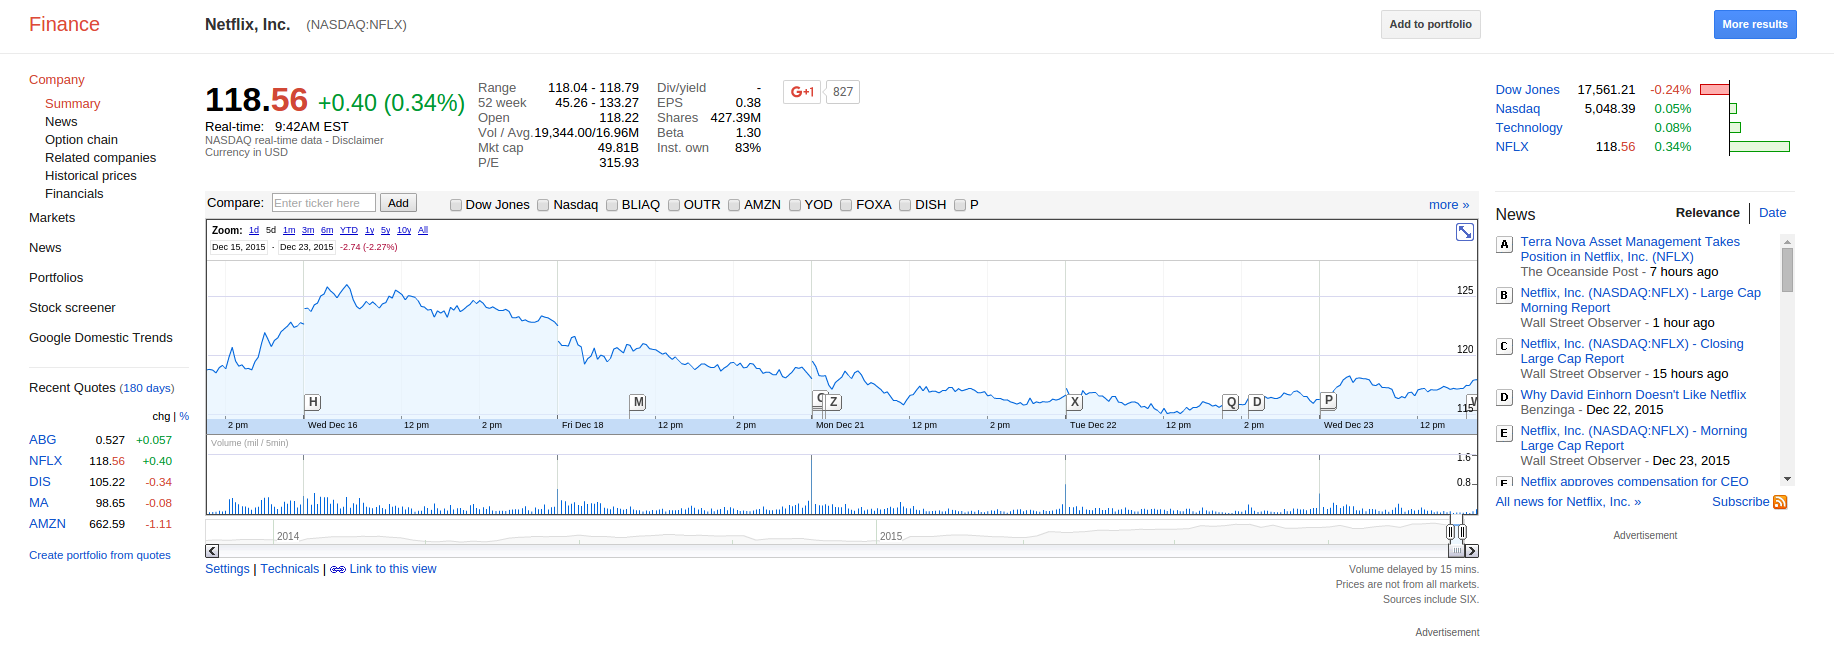
\includegraphics[width=1.2\textwidth]{img/netflix.png}
\label{fig:netflix}
\end{center}
\end{adjustwidth}

Si nos fijamos en la silueta de la gráfica mostrada podemos ver que el precio de las acciones subió hace cuatro días pero ha ido bajando desde entonces. Esta silueta nos permite ver la situación de la empresa cuyo precio en el mercado ha bajado recientemente.

No obstante, podemos ver que la figura no es suave en absoluto sino que oscila constantemente. Estas oscilaciones se deben a la compra y venta de acciones que se produce constantemente.

Cuando el precio de la acción baja, y los corredores de bolsa consideran que ha bajado lo suficiente, comienzan a comprarse acciones lo que hace que la demanda suba y con ella el precio.

Llegados a cierto punto, los accionistas consideran que la acción ha subido lo suficiente de precio y deciden venderla. En este momento la demanda se reduce drásticamente aumentando la oferta con lo que el precio de la acción baja.

Si decidimos invertir en bolsa, debemos estar atentos y tener una óptima conexión de forma que logremos comprar en el momento óptimo (precio mínimo de la acción) y venderla cuando esta alcanza su precio máximo.

\section{Administración}

\subsection{Nóminas, Seguridad Social e IRPF}

Las nóminas financian al Estado a través de dos ``agencias'': la Agencia Tributaria (Hacienda) y la Tesorería General de la Seguridad Social (TGSS).

Un trabajador tiene un salario bruto mensual $S_B$, del que se deduce una cantidad $I_S$ para la TGSS y otra $I_I$ para el IRPF\footnote{Impuesto sobre la Renta de las Personas Físicas, gestionado por la Agencia Tributaria.}. Además, la empresa paga a la TGSS otra cantidad $I_{SE}$ según el salario bruto del trabajador.

\subsubsection{Seguridad Social}

\begin{table}[hbtp]
\centering
\footnotesize
\begin{tabular}{l|r|r|r}
\textbf{Contingencia} & \textbf{Empresa} & \textbf{Trabajador} & \textbf{Total} \\ \toprule
Común - Tipo general & 23.60 & 4.70 & 28.30 \\
Común - Horas extra fuerza mayor & 12.00 & 2.00 & 14.00 \\
Común - Resto horas extra & 23.60 & 4.70 & 28.30 \\ \midrule
Desempleo - Tipo general & 5.50 & 1.55 & 7.05 \\
Desempleo - Contrato temporal a tiempo completo & 6.70 & 1.60 & 8.30 \\
Desempleo - Contrato temporal a tiempo parcial & 6.70 & 1.60 & 8.30 \\ \midrule
Fondo de Garantía Salarial (FOGASA) & 0.20 & 0 & 0.20 \\ \midrule
Formación Profesional & 0.60 & 0.10 & 0.70 \\ \midrule
Accidentes de trabajo y enfermedades profesionales & ($\ast$) & 0 & ($\ast$) \\ \midrule
\end{tabular}
\caption{Tipos (en porcentaje) de cotización, separando qué porcentaje recae en la empresa y qué porcentaje en el trabajador. La parte de ($\ast$) corresponde a la tarifa de primas que varía según trabajador.}
\label{tab:TiposSegSocial}
\end{table}

Las cotizaciones a la Seguridad Social vienen reguladas por la orden ministerial correspondiente de cada año. En 2015, aparecen en la \href{http://www.boe.es/diario_boe/txt.php?id=BOE-A-2015-847}{Orden ESS/86/2015}. Los tipos de cotización se pueden ver en la \fref{tab:TiposSegSocial}.

Las contingencias para accidentes de trabajo y enfermedades profesionales dependen de la empresa y el puesto del trabajador, según la \href{http://www.seg-social.es/Internet_1/Trabajadores/CotizacionRecaudaci10777/TarifadePrimasdeATy48410/index.htm}{tarifa de primas vigente}: se aplica el porcentaje de cotización correspondiente según la actividad económica de la empresa (Cuadro I que aparece en el PDF de la tarifa de primas) salvo que el trabajador entre en alguna de las ocupaciones del Cuadro II de la tarifa de primas, en cuyo caso será el tipo del Cuadro II el que se aplique.

\paragraph{Cálculo de la aportación a la SS} Para el cálculo de la aportación, lo primero que se hace es calcular la base de cotización. Ésta está conformada por el salario bruto, sin contar indemnizaciones o compensaciones de gastos\footnotemark, e incluyendo las pagas extras prorrateadas (esto es, si tenemos dos pagas extras de $x$ euros cada una, al salario bruto para un mes de $d$ días tendremos que añadirle la parte proporcional de las pagas extras, $\frac{d}{365} \cdot 2x $). De este resultado, debemos contar por separado las horas extras y aplicarles el tipo correspondiente de contingencias comunes de la \fref{tab:TiposSegSocial} según sean horas de fuerza mayor (las empleadas para prevenir o reparar siniestros o daños extraordinarios, como terremotos, incendios o similares) o no. El resto de contingencias (desempleo, FOGASA, etc) se aplican al total de salario bruto.

Un detalle a la hora de calcular la base de cotización es que hay \href{http://www.seg-social.es/Internet_1/Trabajadores/CotizacionRecaudaci10777/Basesytiposdecotiza36537/index.htm}{mínimos y máximos de cotización} según puesto y contingencia: si la base no está en ese intervalo, ya sea porque estamos por debajo o por encima, usaremos el mínimo o el máximo respectivamente a la hora de calcular la cuota.

\footnotetext{Ver \href{http://www.seg-social.es/Internet_1/PortalEducativo/Profesores/Unidad6/Cotizacionregimengeneral/Basedecotizacion/Composiciondelabasedecotizacion/index.htm}{la web de la SS} para algunos ejemplos, el \href{http://www.seg-social.es/Internet_1/Normativa/095235?ssSourceNodeId=292}{artículo 23 del Reglamento general sobre cotización y liquidación de 1995 (que supongo sigue vigente)} para el reglamento concreto y \href{http://www.seg-social.es/prdi00/groups/public/documents/binario/178628.pdf}{este boletín de la SS} para una tabla con las deducciones concretas.}

\subsubsection{IRPF}

Cada año (más concretamente, cada ejercicio fiscal), las personas físicas deben hacer la declaración de la renta\footnote{Sólo es obligatorio habiendo recibido más de 22.000 euros brutos de un pagador o más de 11.200 euros de dos pagadores, con el segundo y siguientes pagando más de 1.500 euros.} y pagar un impuesto en base a los ingresos (renta) que haya tenido.

Para evitar el susto en la declaración, las actividades económicas están sujeta a retención. Así, cuando un empleador paga a un empleado, una parte se va a Hacienda retenida en concepto de IRPF\footnotemark. 
Es en la declaración de la renta donde se echan cuentas y se ve si hemos pagado de más o de menos a Hacienda.

\footnotetext{\href{http://www.agenciatributaria.es/static_files/AEAT/Contenidos_Comunes/La_Agencia_Tributaria/Informacion_institucional/Campanias/IRPF_permanente/Informacion_general/Cuestiones_destacadas/reten_ingresos_cuenta_IRPF.pdf}{Aquí los tipos de retención} según la actividad económica, y aquí el \href{http://www.agenciatributaria.es/AEAT.internet/Inicio/La_Agencia_Tributaria/Campanas/Retenciones/Ejercicio_2015__hasta_11_de_julio__o_en_su_caso__31_de_julio_/Informacion_tecnica/Informacion_tecnica.shtml}{algoritmo concreto} (horrible) que usan. En la \href{http://www.agenciatributaria.es/AEAT.internet/Retenciones.shtml}{Agencia Tributaria} está el resto de información necesaria, como un simulador de retenciones.}

La cantidad a pagar a Hacienda depende de un montón de aspectos\footnote{Cosas que deberían aparecer todas en la \href{https://www.boe.es/buscar/act.php?id=BOE-A-2006-20764&tn=1&vd=&p=20151030}{Ley 35/2006} sobre el IRPF y sus sucesivas modificaciones (\href{http://www.boe.es/diario_boe/txt.php?id=BOE-A-2015-7765}{la última, de 2015}.)}. 
La \study{base imponible} se calcula como la \substudy{suma de nuestros ingresos declarados (sin incluir las cotizaciones a la Seguridad Social), quitando los que estén exentos (por ejemplo, ayudas, subvenciones).} De esa base imponible se quita el \substudy{mínimo personal y familiar}, que como mínimo es de 5.550 euros y depende de los hijos que tenga uno a su cargo, discapacidades y demás\footnote{Ver artículos 56 a 60 de la \href{https://www.boe.es/buscar/act.php?id=BOE-A-2006-20764&b=29&tn=1&p=20141128}{Ley del IRPF}.}.

Además, a partir de la reforma fiscal que entra en vigor en 2015, se añade una partida más en concepto de ``gastos generales''\footnote{Ver artículo 19.2.f) de la \href{https://www.boe.es/buscar/act.php?id=BOE-A-2006-20764&b=29&tn=1&p=20141128}{Ley del IRPF}.}, de tal forma que además del mínimo, hay que restar 2.000 euros más de la base imponible (así que pagamos menos impuestos).

\begin{table}[hbtp]
\centering
\footnotesize
\begin{tabular}{r|r|r|r|r}
\textbf{Desde} & \textbf{Hasta} & \textbf{Longitud tramo} & \textbf{Cuota íntegra} & \textbf{Tipo aplicable} \\ \toprule
0 & 12,450 & 12,450 & 0.00 & 19.5 \\
12,450 & 20,200 & 7,750 & 2,427.75 & 24.5 \\
20,200 & 34,000 & 13,800 & 4,326.50 & 30.5 \\
34,000 & 60,000 & 26,000 & 8,535.50 & 38.0 \\
60,000 & $\infty$ & $\infty$ & 18,415.50 & 46.0 \\
\end{tabular}
\caption{Tramos del IRPF para el ejercicio fiscal 2015.}
\label{tab:Tramos2015IRPF}
\end{table}

Lo que nos quede es lo que se llama la base liquidable, a la que se aplica el impuesto según la escala de la \fref{tab:Tramos2015IRPF}, aplicando a cada tramo el porcentaje correspondiente. Por ejemplo, si nuestra base liquidable 30,000 euros una vez quitado el mínimo personal, los primeros 12,450 están gravados al 19.5 \%, los siguientes 7,750 (hasta 20,200) lo están al 24.5 \% y el resto están al 30.5 \%. 
El porcentaje de impuesto efectivo no es por lo tanto el del tramo en el que esté tu base liquidable, sino la media ponderada según los tramos.

Lo de la cuota íntegra es simplemente una ayuda para calcularlo: la cuota íntegra de un tramo es el resultado de aplicar a todos los tramos anteriores su gravamen correspondiente, de tal forma que sólo tengas que calcular el porcentaje para lo que lleves del último tramo y sumarle la cuota íntegra.

\subsubsection{Cuánto paga la empresa}
Hay que destacar que no sólo es el trabajador el que paga el impuesto de la Seguridad Social y el IRPF. Por cada pago que realiza el trabajador (que, como se ha explicado con anterioridad, es pagado directamente por la empresa sustrayendo el importe correspondiente del salario del trabajador), la empresa también tiene que pagar una cantidad, tanto de impuesto de Seguridad Social como IRPF aún mayor que lo que paga el trabajador.

La \fref{tab:EjemploNomina} muestra un ejemplo de nómina de un trabajador, viendo cuánto cobra en neto y cuánto tiene que pagar la empresa.\footnote{Esta tabla se ha obtenido a partir de las transparencias de la asignatura y ha sido completada de acuerdo a las cuentas que se hicieron en clase.}

\begin{table}[hbtp]
\centering
\begin{tabular}{l||r|r||r|r}
\multicolumn{1}{c}{} & \multicolumn{2}{c}{\textit{Trabajador}} & \multicolumn{2}{c}{\textit{Empresa}} \\ \toprule
\textbf{Concepto} & \textbf{Mensual} & \textbf{Anual} & \textbf{Mensual} & \textbf{Anual} \\ \toprule
Salario Bruto & 1.285,71 \texteuro & 18.000,00 \texteuro & 1.285,71 \texteuro & 18.000,00 \texteuro \\
Seguridad Social & 95,25 \texteuro & 1143,00 \texteuro & 465,00 \texteuro & 5.580,00 \texteuro \\
IRPF & 160,07 \texteuro & 2.241,00  \texteuro & 0,00 \texteuro & 0,00 \texteuro \\ \bottomrule
Neto & 1.030,39 \texteuro & 14.616,00 \texteuro & 1750,71 \texteuro & 23.580,00 \texteuro
\end{tabular}
\caption{Un ejemplo de nómina, con tipo de IRPF 12,45\% y Seguridad Social de 6,35\% a cargo del trabajador y 31\% a cargo de la empresa.}
\label{tab:EjemploNomina}
\end{table}

Es decir, si el trabajador recibe un neto de 1.030,39 \texteuro \ al mes, la empresa debe pagar un total de 1750,71 \texteuro \ al mes y el estado recibe 720.32 \texteuro\  cada mes.

\paragraph{Cálculo efectivo del tipo de IRPF}

% % % No entiendo nada.

Vemos que el tipo aplicado de IRPF es $12.45\%$. 

El salario bruto son 18000\texteuro\ . Para calcular el tipo de IRPF calculamos la base imponible:
\[
B_l = 18.000 - \underbrace{5.500 - 2.000 - 1.143}_{8.643} = 9.357,00
\]

Como no sobrepasamos los 12.450 \texteuro\ del primer tramo, se les aplica un $19.5\%$, con lo que el tipo de IRPF será la media ponderada:

\[
	% % Según como lo ha hecho en el examen sería: \frac{8.643*0\% + 6.950*19,5\% + 2425*24,5\%}{18000} = 10.83
	\frac{8.643·0\% + 9.357·19,5\%}{18000} = 10,156\%
\]

Casi exactamente lo obtenido en la tabla.


\subsection{Facturación, ventas y cobros. IVA}

Una factura es, formalmente, un documento con toda la información de una compraventa. Lo emiten los que pueden vender, esto es, autónomos o empresas. La factura siempre ha de incluir el IVA correspondiente a lo que se venda, según los \href{http://www.agenciatributaria.es/static_files/AEAT/Contenidos_Comunes/La_Agencia_Tributaria/Segmentos_Usuarios/Empresas_y_profesionales/Novedades_IVA_2014/Nuevos_tipos_IVA.pdf}{tipos que establezca la AEAT} (principalmente hay tres: general del 21 \%, reducido del 10 \% y superreducido del 4 \%).

El IVA, \concept{Impuesto\IS sobre el Valor Añadido}\index{IVA}, es un impuesto que recae sobre el consumidor, y que gestionan los autónomos y empresas para el Estado. Cuando le vendemos un producto a un consumidor, le cobramos el precio que queramos y además le pedimos un porcentaje de ese precio en concepto de IVA. 
Esa cantidad va directa al Estado en la \study{declaración trimestral del IVA}.

Cuando la venta se la hacemos a otra empresa o autónomo (esto es, no a un consumidor), seguiremos cobrándole el IVA igualmente y dándoselo al Estado. El otro deberá luego deducirse esa cantidad de IVA que nos ha pagado en su declaración del IVA, para que el Estado se la devuelva\footnote{En la práctica no se devuelve, simplemente miran cuánto IVA ha pagado la empresa y cuánto ha cobrado y le ingresa a Hacienda la diferencia - normalmente, las empresas cobran más IVA que el que pagan.}.

Esto desencadena en algunos problemas como nos muestra el siguiente ejemplo, utilizado por el profesor en clase en diversas ocasiones:
\begin{example}
Si desarrollas un Software para el Corte Inglés y quieres ganar $X$ cantidad de dinero con él, se lo tendrás que vender al cliente por el precio $X+$IVA$\times X$.

No obstante, puesto que el Corte Inglés va a deducirse el IVA, es decir, le van a reembolsar lo que te pague de IVA, le interesa recibir esa ``devolución'' antes de haber pagado.

Por tanto, el IVA te exigirá la emisión de la factura lo antes posible aunque la empresa no va a pagarte hasta, por lo menos, un año más tarde.

Puesto que la factura ya ha sido emitida, el Corte Inglés ya puede deducirse el supuesto IVA (que aún no ha pagado) con lo que el Estado le paga. El problema es que esto también implica que tu, como cliente, debes pagar tu IVA (el que le ibas a cobrar al Corte Inglés), aunque este no haya pagado.

Es decir, le vendes un Software a una gran empresa y no sólo tardarás en cobrar sino que, además, deberás pagar el IVA de un beneficio que aún no has percibido.
\end{example}

A raíz de situaciones como la del ejemplo, el estado trató de cambiar las cosas, permitiendo al autónomo del ejemplo no pagar el IVA hasta que recibiera el cobro. No obstante, esto implicaba que el Corte Inglés tampoco recibiría ese IVA hasta pagar.

Finalmente muy pocos autónomos o pequeñas empresas se acogieron a esta posibilidad puesto que esto les implicaba que grandes empresas como el Corte Inglés en el ejemplo, dejasen de contratar sus servicios.

\obs La declaración del IVA se realiza de manera trimestral.

A la pregunta sobre si se ha de facturar o no, la respuesta es sencilla. Si se trata de ingresos esporádicos, no muy grandes y a particulares, teniendo en cuenta el engorro y los costes de hacerse autónomo, lo mejor es buscar formas alternativas de declarar esos impuestos. Si no, probablemente necesites hacerte autónomo. En cualquier caso, siempre hay que declarar los ingresos y pagar los impuestos correspondientes.

\subsection{Certificados digitales}

Bueno, esto no merece mucha explicación. Las administraciones públicas emiten certificados digitales (hay que pedirlo y luego personarse en la administración que corresponda con documentos que acrediten tu identidad como persona física o jurídica) para operar con ellas a través de Internet.

A estas alturas de la carrera, todo informático que se precie debe entender perfectamente qué son los certificados digitales y cómo funciona.

\subsection{Contratos}

\begin{table}[hbtp]
\centering
\begin{tabular}{l|l|l}
\textbf{Despido} & \textbf{Días por año trabajado} & \textbf{Mensualidades máximas} \\ \toprule
Procedente & 20 & 12 \\
Disciplinario & 0 & 0 \\
Improcedente & 33 & 24 \\
Fin contrato temporal & De 8 a 12 & - \\
\end{tabular}
\caption{Tabla con las indemnizaciones por despido.}
\label{tab:Despido}
\end{table}

Los contratos pueden ser de diferentes tipos, principalmente se dividen en fijos y temporales (estos pueden ser por obra y servicio, por tiempo...). También hay contratos de formación y de prácticas.

Una vez que se contrata a un empleado, se le puede despedir\footnote{Un despido es una anulación del contrario por parte del contratante} previo pago de la correspondiente indemnización, que dependerá, entre otros, del tiempo que se trabaje (días por año trabajado, añadiendo la parte proporcional a los períodos inferiores a un año) y el tipo de despido, según la \fref{tab:Despido}. 
Describimos a continuación los \study{tipos de despido}\footnote{Ver la sección cuarta del \href{https://www.boe.es/buscar/act.php?id=BOE-A-1995-7730&tn=1&p=20151024}{Estatuto de los trabajadores}}:

\begin{itemize}
\item \concept{Despido\IS procedente}. Se extingue el contrato por ineptitud del trabajador conocida o sobrevenida después de la contratación y del período de prueba, por faltas de asistencia o por faltas de adaptación a cambios razonables en el puesto de trabajo. También se podrá efectuar un despido por causas económicas de la empresa.
\item \concept{Despido\IS disciplinario}. Se extingue el contrato por incumplimiento grave y culpable del trabajador, como faltas repetidas e injustificadas, indisciplina, ofensas verbales o física, acoso y similares.
\item \concept{Despido\IS improcedente}. Cuando se modifiquen las condiciones de trabajo del empleado sustancialmente sin respetar el artículo 41 del Estatuto de los trabajadores, falta de pago u otro incumplimiento grave del empresario (el trabajador tendrá que solicitar en el juzgado de lo social la extinción). También habrá despido improcedente si un juez lo determina así.
\end{itemize}

Además, cuando se acaba un contrato temporal, e trabajador tendrá derecho a doce días de salario por cada año de servicio\footnote{Ver \href{http://www.empleo.gob.es/es/Guia/texto/guia_7/contenidos/guia_7_16_4.htm}{la web del Ministerio de Empleo} para los detalles exactos.}.

\section{Análisis de estados financieros}

\begin{defn}[Contabilidad]
La contabilidad se puede definir, en palabras del profesor, como una técnica que permite construir e interpretar estados financieros.
\end{defn}

El análisis de estados financieros de una empresa implica, como su nombre indica, analizar y diseccionar el estado del dinero en una empresa. Se podrían distinguir dos ámbitos de contabilidad:

\begin{itemize}
\item \textbf{Contabilidad financiera}. Es un registro sistemático de las operaciones que la empresa realiza con el exterior.

Forman parte de la contabilidad financiera, por ejemplo, los préstamos pedidos, la compra de material, los pagos a Hacienda, las ventas, la compra de edificios, ...

Esta contabilidad se lleva con el objetivo de llevar un control y \textbf{es obligatoria}. Sirve para conocer el patrimonio de la compañía y los resultados de la empresa.

Si bien algunos conceptos pueden ser ambiguos a la hora de estudiarlos, existen una serie de \textbf{estándares} que nos dicen cómo proceder.

\item \textbf{Contabilidad de costes} Tiene como objetivo conocer los costes, los márgenes de beneficios y las contribuciones de los socios.

En general depende enormemente de la estructura interna de la empresa por lo que no está estandarizada y no existen programas informáticos que ayuden en esta tarea.
\end{itemize}

En esta sección nos centraremos en el estudio de la \textbf{contabilidad financiera}.

\subsection{Contabilidad: Balance, PyG y caja}
\label{sec:Contabilidad}

Las empresas españolas están obligadas a presentar las cuentas anuales en el registro mercantil según el \href{https://www.boe.es/buscar/doc.php?id=BOE-A-2007-13023}{Plan General Contable de 2007}, corregido en la \href{https://www.boe.es/boe/dias/2009/02/10/pdfs/BOE-A-2009-2276.pdf}{Orden JUS/206/2009 del 28 de enero}.

\subsubsection{Técnica de contabilidad: Asientos}

\begin{table}[hbtp]
\centering
\begin{tabular}{r|p{5cm}||p{5cm}|l}
\textbf{Debe} & \textbf{Concepto} & \textbf{Concepto} & \textbf{Haber} \\ \toprule
1.096,25 & (640) Sueldos y salarios & (476) Organismos de la Seg. Social. acreedores & 480,81 \\
372,63 & (642) S.S. a cargo de la empresa & (4751) Hac. Pública acreedor por retenciones practicadas & 94,27 \\
 & & (465) Remuneraciones pendientes de pago & 893,8 \\ \midrule
 893,8 & (465) Remuneraciones pendientes de pago & (572) Bancos c/c & 893,8 \\ \midrule \midrule
10.000 	& (600) Compra de mercaderías & (400) Proveedores &	12.100 \\
2.100 	& (472) H.P. IVA Soportado & &  \\ \midrule
12.100 	& (400) Proveedores & (572) Bancos e instituciones bancarias &	12.100 \\ \midrule \midrule
12.100 	& (430) Clientes & 	 (700) Venta de mercaderías & 10.000 \\
 & & (477) H.P. IVA Repercutido & 2.100 \\ \midrule
12.100 & (572) Bancos c/c & (430) Clientes & 12.100 \\
 \bottomrule
\end{tabular}
\caption{Ejemplo de asientos contables. El primer asiento corresponde al pago de un salario: sale dinero de la cuenta de sueldos y salarios (lo que en el PyG aparecerá como sueldos y salarios) y de la cuenta de la seguridad social a cargo de la empresa. Ese dinero se va a la Seguridad Social (la parte de cotización de la SS de la empresa y la parte del trabajador), a la hacienda pública (el IRPF retenido) y a remuneraciones pendientes de pago. En el siguiente asiento, sacamos las remuneraciones pendientes de pago y las pagamos a través del banco. En los dos siguientes asientos, hacemos una compra de material. El tercer grupo de asientos es un ejemplo de cómo contabilizaríamos una venta pagada por entidad bancaria (si fuese al contado, en lugar de Bancos tendríamos Caja). En los dos últimos grupos de asientos, el primer asiento corresponde a cuando se hace la venta, y el segundo a cuando se hace el cobro efectivo.}
\label{tab:Asientos}
\end{table}

La técnica contable lleva la lista de asientos. Un \concept{Asiento} es simplemente el registro de una operación. Cada cuenta tiene dos partes: el lado del debe llamado \textbf{partida} (izquierdo) y el lado del haber llamado \textbf{contrapartida} (derecho). Esto quiere decir que una cuenta puede incrementar o aminorar su saldo según las operaciones que se realicen. Estos aumentos y disminuciones tienen un nombre: \concept{Cargo} y \concept{Abono}. \href{http://www.plangeneralcontable.com/?tit=guia-de-contabilidad-para-torpes&name=GeTia&contentId=man_ctorpes&manPage=8}{En esta página se puede encontrar una descripción más detallada de estos conceptos}.

De manera obvia si alguien gana es porque otro lo pierde. Nuestro objetivo al estudiar la contabilidad es saber quién gana, quién pierde y qué consecuencias tiene esto. Este es el principio de \textbf{partida doble}.

Las cuentas de donde sale y entra el dinero están definidas según el PGC\footnote{\href{https://www.boe.es/boe/dias/2007/11/20/pdfs/C00001-00152.pdf}{Plan General de Contabilidad}.}. La \fref{tab:Asientos} tiene un ejemplo con varias operaciones y su descripción.

%Adicionalmente, sería relevante revisar qué pasa con las cuentas de bancos y de otros activos en general. La cuestión es que cuando una cuenta de activo aparece en el ``debe'', esta cuenta aumenta (por ejemplo, cuando ponemos la cuenta de Bancos en el debe, significa que nuestro activo por dinero en bancos aumenta), y disminuye cuando aparece en el haber. Análogamente, cuando una cuenta de pasivo aparece en el haber, su cantidad aumenta; y si aparece en el debe, su cantidad disminuye.

Al final, todos esos asientos se suman (el haber es positivo, el debe es negativo) y sale la \concept{Mayor}. El debe y el haber deberían sumar lo mismo al hacer el mayor de todas las cuentas ya que, de no ser así, significaría que estamos creando dinero de la nada.

En el apéndice \ref{sec:contabilidad} podemos encontrar un esquema que resume los conceptos que acabamos de ver sobre la \textbf{contabilidad}, acompañado de un ejemplo.

\subsubsection{Determinación de rendimientos para el IRPF}

Cuando uno lleva a cabo una actividad económica (esto es, es autónomo), tenemos dos formas\footnotemark de estimar nuestros rendimientos netos y por lo tanto dos métodos de decirle a Hacienda cuál es nuestra base imponible sobre la que se aplican los impuestos.

\footnotetext{Esto aparece en el \href{https://www.boe.es/buscar/act.php?id=BOE-A-2006-20764}{artículo 16.2 de la ley del IRPF}, y se desarrollan los regímenes en el \href{https://www.boe.es/buscar/act.php?id=BOE-A-2007-6820}{artículo 27 del Real Decreto 439/2007}.}

Existen dos regímenes de estimación: la directa (con dos modalidades) y la objetiva.

El \concept{Régimen\IS de estimación directa simple} es el método por defecto, que sólo deja de aplicarse si renunciamos a él o si la cifra de negocio (las ventas que tenemos quitadas deducciones e IVA\footnote{Definido en el \href{http://www.boe.es/buscar/doc.php?id=BOE-A-1989-30361}{artículo 191 de un RDL derogado}, aunque parece que la cifra no ha cambiado.}) supera los 600.000 euros anuales. La base imponible se calcula como los ingresos menos los gastos y deducciones, incluyendo además una deducción del 5\% del rendimiento neto del ejercicio anterior para provisiones y gastos de difícil justificación. Hay además \href{http://portal.circe.es/es-ES/emprendedor/EmpresarioIndividual/TributacionAutonomos/Paginas/AutonomoEstimacionDirectaSimplificada.aspx}{otros pequeños detalles}.

El \concept{Régimen\IS de estimación directa normal} vale cuando la cifra de negocio supera los 600.000 euros anuales de antes. En estos casos la base imponible se calcula igual pero añadiendo el autoconsumo\footnote{Ver \href{http://www.pymesyautonomos.com/fiscalidad-y-contabilidad/el-autoconsumo-de-bienes-y-servicios-tratamiento-fiscal-y-contable}{este sitio} para una explicación, básicamente es cuando el autónomo consume sus propios servicios.} a los ingresos. \href{http://portal.circe.es/es-ES/emprendedor/EmpresarioIndividual/TributacionAutonomos/Paginas/autonomoestimacionDirectaNormal.aspx}{Aquí hay más detalles}.

Estos dos casos requieren que el autónomo lleve control de su contabilidad. No obstante, en ocasiones, esto escapa de la formación/preparación del autónomo en cuestión.

Por ejemplo, en el caso de un taxista, es frecuente que no lleve un control detallado de la contabilidad y por tanto sea incapaz de acogeres a uno de los dos métodos de estimación del IRPF que acabamos de ver.

Para casos como este, Hacienda tolera que algunas personas no lleven la contabilidad de su negocio (ya sea porque no pueden o porque no quieren hacerlo). En estos casos es Hacienda la que calcula, en lugar del propio autónomo, cuáles son sus ganancias.

Como hacienda no tiene datos sobre la situación real del negocio, lo que hace es una estimación basándose en estadísticas y en variables objetivas del negocio. Esto es lo que se conoce como \textbf{régimen} de estimación objetiva.


El \concept{Régimen\IS de estimación objetiva}\footnote{Regulado en el \href{https://www.boe.es/buscar/act.php?id=BOE-A-2007-6820}{artículo 32 del RDL 439/2007}.} se puede aplicar sólo cuando la cifra de negocio\footnote{Para la cifra de negocio debe incluirse la del cónyuge, descendientes y ascendientes que realicen actividades económicas similares.} no supera los 150.000 euros anuales (250.000 para actividades agrícolas, ganaderas y forestales), y siempre y cuando el importe de facturas emitidas a profesionales o empresarios (es decir, a consumidores habituales) no supere los 75.000 euros. Además, el volumen de las compras en bienes y servicios, excluidas las adquisiciones de inmovilizado, en el ejercicio anterior no puede superar la cantidad de 150.000 euros anuales. El cálculo de esto se hace en base a estimadores y diversos parámetros (número de empleados, de repartidores, superficie del local) según diga la normativa correspondientes. Lo malo es que estos coeficientes son pre-crisis y por lo tanto están algo desajustado de la realidad.% TODO.

\begin{example}
Veamos un ejemplo de situación real descrita por el profesor en clase.

En un determinado barrio tenemos dos farmacias. Una de ellas situada en la calle principal, lo que presumiblemente le da ventaja respecto a otros establecimientos y goza de una amplia superficie.

Por otro lado tenemos otra farmacia de aspeco más modesto situada en una calle paralela a la principal, con una clara menor afluencia de viandantes.

Debido a mal o buen caracter de los propietarios de las farmacias resulta que la segunda acapara casi toda la clientela del barrio.

En esta situación, a la primera farmacia le interesa llevar su contabilidad, de forma que pueda cotizar en función de lo poco que gana. Si decidiera emplear un régimen de estimación objetiva tendría problemas puesto que las ventas medias que se le presuponen son superiores a las que tiene y ciertos datos objetivos como la dimensión del local o la posición del establecimiento jugarían en su contra.

Por el contrario, a la segunda farmacia le interesa la estimación objetiva pues sus beneficios se sitúan por encima de la media y los aspectos objetivos como el tamaño o la posición del local juegan a su favor.
\end{example}

\paragraph{Moduleros}

Con este término nos referimos a aquellas personas que se dedican a emitir facturas falsas. \textbf{Evidentemente esta práctica está fuera de la ley}. Estas personas cotizan por el régimen de estimación objetiva, de modo que no tienen por que llevar su contabilidad y, por ello, Hacienda no tiene nada que controlar.

Así estas personas no tienen ningún problema en vender un producto, que normalmente vendería a 100 \text{euro} a 200 \texteuro, emitiendo una factura de 1000 \texteuro, lo que permite al comprador recuperar el IVA que supuestamente ha pagado, es decir, recupera 210 \texteuro.

En un ejemplo tan simple como acabamos de ver todos los implicados salen ganando salvo \textbf{Hacienda}.

\subsubsection{Balance}

Hay tres formas de afrontar la contabilidad de la empresa. La primera es la que surge al mirar el patrimonio de una empresa, que es donde vemos el activo $A$ y el pasivo $P$ (lo que se tiene y lo que se debe) y el patrimonio neto $N$. Este último a veces se denomina pasivo no exigible. En cualquier caso, las tres cantidades están relacionadas por la siguiente fórmula:
\[ A - P = N\]

\begin{figure}[hbtp]
\centering
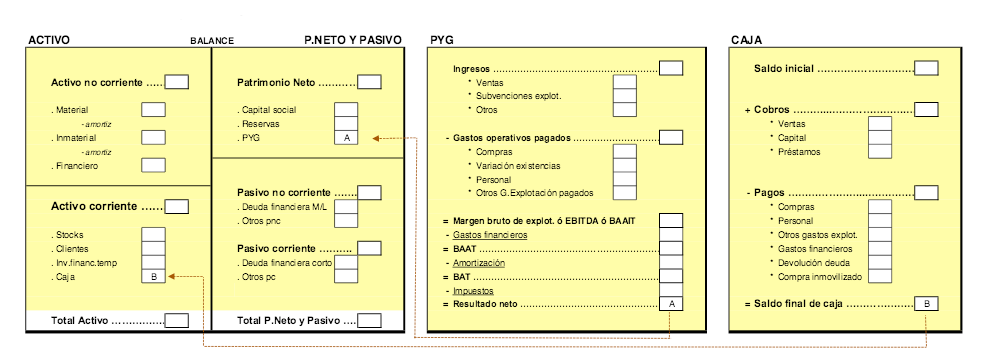
\includegraphics[width=\textwidth]{img/Balance_PyG_Caja.png}
\caption{Un ejemplo de modelo de balance, PyG y caja extraído de \href{http://maestremiranda.com/techdir/wp-content/uploads/2015/10/EF0.-Bal_PYG_Caja.pdf}{maestremiranda.com}}
\label{fig:BalancePyGCaja}
\end{figure}

La \fref{fig:BalancePyGCaja} contiene una muestra de qué cuenta dentro de activos y qué dentro de pasivos. La diferencia entre activo o pasivo corriente y no corriente es sencilla: lo corriente es lo volátil, lo que está a corto plazo.

La \fref{tab:Balance} tiene un modelo abreviado del balance del Plan General Contable de 2007, relleno con los datos del siguiente ejemplo, extraído de las transparencias del profesor empleadas en las clases de teoría:

\begin{itemize}
\item En tesorería (cuentas corrientes) dispone de 260 (\textit{Efectivo y otros activos líquidos}).
\item Durante el ejercicio ha obtenido 10 de beneficio (\textit{PyG}).
\item Se sabe que hay una póliza de préstamo bancario por 230 (\textit{Deuda M/L}).
\item La aportación inicial de los socios fue de 100 (\textit{Capital social}).
\item A los suministradores todavía les debe 10 (letra a pagar con vencimiento 30 días) (\textit{Acreedores comerciales / proveedores}).
\item Los productos en inventario se valoran en 20 (\textit{Existencias}).
\item El activo fijo (mobiliario y ordenadores) asciende a 20 (\textit{Inmovilizado material}).
\item La cifra acumulada de beneficios retenidos es de 50 (\textit{Reservas}).
\item De las ventas realizadas le faltan por cobrar 100 (un cliente debe por mercancía no pagada) (\textit{Deudores comerciales}).
\end{itemize}

\begin{table}[hbtp]
\begin{minipage}{\textwidth}
\footnotesize
\centering
\begin{tabular}{l|c|c}
\textbf{Concepto} & \textbf{Debe} & \textbf{Haber} \\ \toprule
\multicolumn{3}{c}{\textsc{Activo} - \textbf{A) Activo no corriente}} \\ \midrule
I. Inmovilizado intangible & & - \\
II. Inmovilizado material & & 20 \\
III. Inversiones inmobiliarias & & - \\
IV. Inversiones en empresas del grupo y asociadas a largo plazo & & - \\
V. Inversiones financieras a largo plazo & & - \\
VI. Activos por impuesto diferido\footnote{Lo que el Estado nos debe de impuestos.} & & - \\
\textbf{Total activo no corriente} & & \textbf{20} \\ \midrule
\multicolumn{3}{c}{\textsc{Activo} - \textbf{B) Activo corriente}} \\ \midrule
I. Activos no corrientes para la venta & & - \\
II. Existencias & & 20 \\
III. Deudores comerciales y otras cuentas a cobrar & & 100 \\
IV. Inversiones en empresas del grupo y asociadas a corto plazo & & - \\
V. Inversiones financieras a corto plazo & & - \\
VI. Periodificaciones a corto plazo\footnote{Pagos hechos pero no devengados. Por ejemplo si se paga una póliza de seguros de dos años, la parte correspondiente al año siguiente debería ir en este epígrafe para compensar.} & & - \\
VII. Efectivo y otros activos líquidos equivalentes & & 260 \\
\textbf{Total activo corriente} & & \textbf{380} \\ \midrule
\multicolumn{3}{c}{\textsc{Patrimonio neto} - \textbf{A-1) Fondos propios}} \\ \midrule
I. Capital suscrito & & 100 \\
II. Prima de emisión\footnote{La diferencia entre el valor nominal de las acciones y el que se obtiene por ellas.} & & - \\
III. Reservas\footnote{Hay una obligación legal de manterla con cargo a los beneficios (10 \% cada año) hasta que alcance el 20\% del capital social. Sólo se podrá usar para compensar pérdidas. Si se quiere, se puede dotar por encima de ese valor, pero nunca podrá bajar del 20\% del C.S.} & & - \\
IV. Acciones y participaciones en patrimonio propias & & - \\
V. Resultados de ejercicios anteriores & - & 50 \\
VI. Otras aportaciones de socios & & - \\
VII. Resultado del ejercicio (PyG) & & 10 \\
VIII. Dividendo a cuenta & - &\\
IX. Otros instrumentos de patrimonio neto & - & - \\
\textbf{Total fondos propios} & - &  \textbf{160} \\
\textbf{A-2) Ajustes por cambio de valor} & - & - \\
\textbf{A-3) Subvenciones, donaciones y legados} & & - \\ \midrule
\multicolumn{3}{c}{\textsc{Pasivo} - \textbf{B) Pasivo no corriente}} \\ \midrule
I. Provisiones a largo plazo\footnote{Las provisiones son partidas que tendremos que pagar (sueldos, impuestos) más tarde, con importe o fecha no concretos.} & - &  \\
II. Deudas a largo plazo & 230 & \\
III. Deudas con empresas del grupo y asociadas a largo plazo & - &  \\
IV. Pasivos por impuesto diferido & - &  \\
V. Periodificaciones a largo plazo &  & \\
\textbf{Total pasivo no corriente} & \textbf{230} &  \\ \midrule
\multicolumn{3}{c}{\textsc{Pasivo} - \textbf{B) Pasivo corriente}} \\ \midrule
I. Pasivos vinculados con activos no corrientes mantenidos para la venta & - & \\
II. Provisiones a corto plazo & - & \\
III. Deudas a corto plazo  & - & \\
IV. Dedudas con empresas del grupo y asociadas a corto plazo & - & \\
V. Acreedores comerciales y otras cuentas a pagar & 10 & \\
VI. Periodificaciones a corto plazo & - & \\
\textbf{Total pasivo corriente} & \textbf{10} &  \\ \midrule
\end{tabular}
\caption{Modelo abreviado de balance relleno con el ejemplo anterior, según el Plan General Contable 2007. Se puede ver que $P = 240$, $A = 400$, $N = 160$ así que todo cuadra.}
\label{tab:Balance}
\end{minipage}
\end{table}

\paragraph{\concept{Gastos\IS Activados}} Una cosa que quizás merece la pena mencionar porque aparece en el ejemplo de balance de Terra y Jazztel, comentado en clase y que podemos ver en la figura \fref{fig:TerraJazztel}. Cuando se gasta dinero en I+D, existe la posibilidad de ``activar'' esos gastos, esto es, pasarlos en el balance como activo, más concretamente inmovilizado intangible, si se cumplen unas ciertas condiciones\footnote{Rentabilidad asegurada en cinco años o menos. Si son gastos de desarrollo, se puede demostrar que se van a amortizar a lo largo de más años.}. Si no se activasen, los gastos de desarrollo irían como pérdidas directamente.

\begin{figure}[hbtp]
\centering
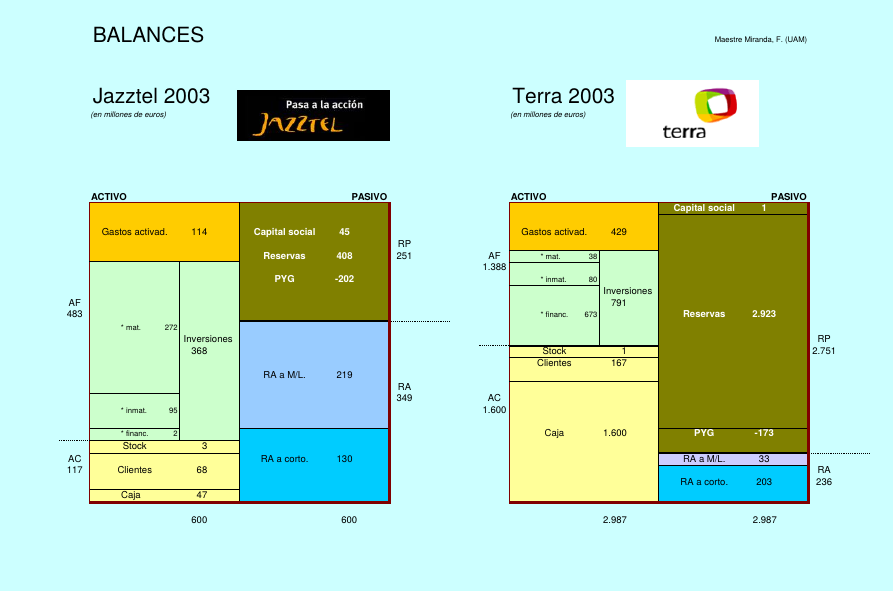
\includegraphics[width=\textwidth]{img/TerraJazztel.png}
\caption{Ejemplo de balance de las compañías Terra y Jazztel respectivamente.}
\label{fig:TerraJazztel}
\end{figure}

¿En qué consiste exactamente esto? La idea es que se puedan distribuir los gastos de un proyecto a lo largo del tiempo. En lugar de dejar que los gastos se vayan directamente a la cuenta de beneficios y nos provoquen pérdidas, añadimos una ganancia en la cuenta 3 (Trabajos realizados por la empresa para su activo, ver la \fref{tab:PyG}) que cancele esos gastos y que aumente la partida de inmovilizado intangible en nuestro balance.

Según el PGC, los gastos de I+D deben amortizarse en un plazo de cinco años. Es decir, que podemos retrasar el momento de imputar los gastos hasta cinco años: más tarde tendrán que ir obligatoriamente como pérdidas. La cuestión es cuándo empieza ese plazo. Los gastos de investigación deben amortizarse ya desde el primer momento en el que se activan, pero los de desarrollo\footnote{La diferencia entre desarrollo o investigación es, a grandes rasgos, que el desarrollo va dirigido a una aplicación concreta y no sólo a indagar y ampliar conocimiento.} sólo se deben empezar a amortizar cuando el proyecto acaba.

Esto permite crear proyectos de desarrollo y no contar sus gastos hasta que el proyecto acaba y se puede empezar a vender. En ese caso podremos amortizar los gastos y evitar que aparezcan pérdidas cuando no deben. Por supuesto, esto admite trampas: si nunca terminamos un proyecto de desarrollo y seguimos imputando sus gastos al inmovilizado intangible, estamos enmascarando pérdidas y podemos acabar con un agujero patrimonial curioso.

\subsubsection{Pérdidas y ganancias (PyG)}

Mientras que el balance da una foto instantánea el destado de una empresa, la cuenta de pérdidas y ganancias (PyG) indica cómo varía ese estado a lo largo del tiempo. Es importante recalcar que aquí se usa el criterio de \concept{Devengo}, por el cual los ingresos y gastos computan cuando nos comprometemos a ellos y no cuando el dinero de verdad cambia de manos (por ejemplo, una factura emitida en noviembre va en las cuentas de noviembre aunque nos transfieran el dinero en diciembre).

De nuevo en la \fref{fig:BalancePyGCaja} se puede ver qué hay en cada cosa, aunque de nuevo vamos a hacer un ejemplo. Durante un ejercicio se producen los siguientes hechos:

\begin{itemize}
\item Los sueldos y salarios se elevan a 150.
\item Los intereses de la deuda ascienden a 210.
\item Los servicios generales suman 30.
\item El importe de la cifra de negocio es de 500.
\item Se han dotado 20 para recuperar activos fijos.
\item La tasa impositiva es de un 35\%.
\item Los aprovisionamientos se cifran en 70.
\item El valor del stock final supera el inicial en 60
\end{itemize}

Los resultados se pueden ver en la \fref{tab:PyG}.

\begin{table}[hbtp]
\centering
\begin{minipage}{\textwidth}
\footnotesize
\begin{tabular}{l|c|c}
\textbf{Concepto} & \textbf{Debe} & \textbf{Haber} \\ \toprule
1. Importe neto de la cifra de negocios & & 500 \\
2. Variación de existencias de productos terminados y en curso de fabricación & - & 60 \\
3. Trabajos realizados por la empresa para su activo\footnote{Por ejemplo, I+D. Ver arriba la discusión de gastos activados.} & - & \\
4. Aprovisionamientos & 70 &  \\
5. Otros ingresos de explotación\footnote{Subvenciones, donaciones y legados que financien activos o gastos de la explotación.} & & - \\
6. Gastos de personal & 150 & \\
7. Otros gastos de explotación & 30 & \\
8. Amortización del inmovilizado & - & \\
9. Imputación de subvenciones de inmovilizado no financiero\footnote{Subvenciones, legados y donaciones que financien el activo no corriente (p.e., te regalan una casa).} & - & - \\
10. Exceso de provisiones & - & \\
11. Deterioro y resultado por enajenaciones\footnote{Ventas, que los economistas hablan raro.} de inmovilizado & - & \\ \midrule
\textbf{A) Resultado de explotación} (BAAAIT) ($\sum_1^{11}$) & \textbf{250} & \textbf{560} \\ \midrule
12. Ingresos financieros & & - \\
13. Gastos financieros & 210 & \\
14. Variación de valor razonable en instrumentos financieros & - & - \\
15. Diferencias de cambio\footnote{De divisas, supongo.} & - & - \\
16. Deterioro y resultados por enajenaciones de instrumentos financieros & - & - \\ \midrule
\textbf{B) Resultado financiero} (BAAT) ($\sum_{12}^{16}$) & \textbf{210} & \textbf{0} \\ \midrule
\textbf{C) Resultado antes de impuestos} (BAT) ($A + B$) & \textbf{460} & \textbf{560} \\ \midrule
17. Impuestos sobre beneficios & 35 & \\ \midrule
\textbf{D) Resultado del ejercicio} ($C + 17$) & \textbf{495} & \textbf{560} \\ \bottomrule
\end{tabular}
\caption{Tabla de pérdidas y ganancias: el resultado final es de ganancias de 65. \href{http://www.plangeneralcontable.com/?tit=guia-del-pgc-de-pymes&name=GeTia&contentId=man_pgcpym&manPage=26}{Aquí hay} una explicación algo más detallada de los conceptos. Los \texttt{/BA+I?T/} son abreviaciones que corresponden a beneficios antes de impuestos e intereses. Hay otro \texttt{/BA+I?T/} que corresponde a los beneficios antes de amortizaciones.}
\label{tab:PyG}
\end{minipage}
\end{table}

Un concepto relevante en el PyG es la \concept{Amortización}, que permite ajustar las cuentas considerando la depreciación de los activos. Por ejemplo, si compramos un coche tenemos que tener en cuenta que su precio disminuye con el tiempo. La amortización implica restarle al valor de ese activo un cierto porcentaje cada año. La \href{http://www.boe.es/diario_boe/txt.php?id=BOE-A-2014-12328}{Ley 27/2014} en su artículo 12 (Capítulo II) muestra los porcentajes de amortización para cada tipo de elemento y el período máximo de años que se pueden amortizar.

El balance de pérdidas y ganancias es importante para Hacienda por el \concept{Impuesto\IS de sociedades}: un impuesto sobre los beneficios de las empresas. En España está regulado por la Ley 27/2014, de 27 de noviembre, y es del 30\% para grandes empresas y 25\% para PYMEs, aunque luego en la práctica \href{http://www.agenciatributaria.es/AEAT.internet/Inicio/_Segmentos_/Empresas_y_profesionales/Empresas/Impuesto_sobre_Sociedades/Periodos_impositivos_iniciados_hasta_31_12_2014/Tipos_de_gravamen_aplicables_a_periodos_impositivos_iniciados_en_el_ano_2013_y_2014.shtml}{hay otros tipos contando con reducciones}. En País Vasco y Navarra, que cuentan con el concierto económico y por lo tanto Hacienda propia, los gobiernos autonómicos pueden cambiar los impuestos. Navarra mantiene los tipos del resto de España, mientras que el País Vasco \href{http://www.ogasun.ejgv.euskadi.eus/r51-341/es/contenidos/informacion/6901/es_2316/es_12215.html}{impone tipos reducidos} del 28 \% y 24 \% para grandes empresas y PYMEs respectivamente.

Hablando de \concept{PYMEs}, la definición de qué es una PYME varía según para qué queramos aplicarlo. En el caso que nos ocupa, la Agencia Tributaria, en la ley de antes que regula el IS, considera PYME (o \concept{Entidad\IS de reducida dimensión}) a aquellas que el importe neto de la cifra de negocios en el período inmediato anterior sea inferior a 10 millones de euros\footnote{Hay ciertas condiciones adicionales. Por ejemplo, si una empresa forma parte de un grupo de sociedades (definido en el \href{https://www.boe.es/buscar/act.php?id=BOE-A-1885-6627&tn=1&vd=&p=20150721}{Artículo 42 del Código de Comercio}, básicamente dos empresas pertenecen a un mismo grupo si una de ellas tiene poder sobre la otra en votos o de alguna otra forma) los beneficios que se tienen en cuenta son los de todo el grupo.}. El hecho de ser PYME o no también influye en el tipo de cuentas que deben de presentar. Para este caso, las condiciones están en el PGC\footnote{Ver \href{https://www.boe.es/boe/dias/2009/02/10/pdfs/BOE-A-2009-2276.pdf}{Orden JUS/206/2009 del 28 de enero}.}.



Hemos mencionado el \concept{Importe neto\IS de la cifra de negocios}. ``El importe de la cifra de negocios comprenderá los importes de la venta de los productos y de la prestación de servicios correspondientes a las actividades ordinarias de la Sociedad deducidas las bonificaciones y demás reducciones sobre las ventas, así como el Impuesto sobre el Valor Añadido y otros impuestos directamente relacionados con la mencionada cifra de negocios.  '' (Definición obtenida del \href{http://www.minhap.gob.es/Documentacion/Publico/NormativaDoctrina/Contabilidad%20y%20Auditoria%20de%20Empresas/Contabilidad/cifranegocA.pdf}{BOE 18/01/1992}
) Vamos, básicamente \textbf{los ingresos totales} que realmente se ingresan.

\subsubsection{Caja}

La caja es el estado más sencillo de los tres que hemos visto: refleja el flujo de dinero real en la empresa, pagos y cobros. Lo más sutil es que podemos dividir los flujos en operacionales (relacionados con la explotación, como ventas o compras a proveedores) y no operacionales (por ejemplo, ampliaciones de capital, operaciones financieras, ventas de activos no corrientes o dividendos). El resultado de esto es a veces lo que se llama el \concept{Cash-flow}.

El \textbf{déficit de caja} es un concepto teórico que no puede darse en la vida real. La caja es el capital efectivo del que se dispone. Si hacemos bien las cuentas, cuando no hay dinero en la caja no se puede sacar dinero de la caja.

\obs Mientras que nos interesa tener una PyG lo mayor posible, puesto que esto implica mayores ganancias, con la caja nos interesa tener un resultado lo más cerano a 0. Esto se debe a que el dinero que tengamos en caja es dinero que está ``quieto'' y por tanto no tiene ninguna rentabilidad.

\subsection{Circuito contable integrado}

Uno puede simplificar las cuentas en un circuito contable integrado, cuya única mención en Internet es \href{http://maestremiranda.com/techdir/wp-content/uploads/2015/10/CircuitoContable.pdf}{en maestremiranda.com}. En el apéndice \ref{sec:circuitoContableIntegrado} puede observarse el ejemplo visto en clase completado.

\subsection{Análisis de ratios}

En la \fref{sec:IndicadoresFinancieros} veíamos algunos indicadores financieros. Para analizar el estado de una empresa usaremos algunos de estos, como el ROE (Return on Equity o rentabilidad financiera, beneficios entre recursos propios) o ROI (Return on investments, rentabilidad económica resultado de explotación entre los activos). La \fref{tab:Ratios} tiene un desglose y ejemplos de todos los ratios. En general, todos son fáciles de ver y no merecen una explicación extensa. Sólo algunas aclaraciones:

\begin{itemize}
\item La rentabilidad económica es igual al margen por la rotación (inmediato al ver las fórmulas).
\item La cobertura del inmovilizado, que tiene un nombre un poco malo, se refiere a qué porcentaje del patrimonio de la empresa está cubierto por el activo no corriente, esto es, activos que tenemos pero que no podemos usar directamente para pagar nuestras deudas. Por debajo de uno la empresa está en suspensión de pagos (no tenemos de dónde sacar dinero para pagar nuestras deudas).
\item El ratio de circulante también tiene un nombre cutre. A veces lo llaman ratio de liquidez general. En cualquier caso, sirve para ver qué porcentaje de la deuda a corto plazo se puede atender.
\item El test ácido, que de nuevo tiene un nombre feo (a veces se le llama ratio de liquidez inmediata), es similar al anterior pero se refiere sólo al dinero directo que tenemos y excluye el \textit{stock}, que tendríamos que vender si queremos usarlo para cubrir las deudas.
\item Por último, los ratios que tienen que ver con el pasivo, aunque en una primera pasada podamos pensar que es mejor tenerlos tan altos como sea posible (esto es, tener muy pocas deudas), en realidad no es así según la teoría económica: si tenemos muchos activos, podemos endeudarnos más a coste bajo e invertir más en nuestro negocio para sacar más beneficios y ganar más dinero (bienvenidos al capitalismo).
\end{itemize}

Además de estos ratios existen tres conceptos fundamentales que nos permiten comprender la situación actual de una empresa: \textbf{solvencia}, \textbf{rentabilidad} y \textbf{liquidez}.

Estos conceptos no son fórmulas que nos permitan obtener un valor concreto con el que comprar sino que hacen referencia a características que puede tener o no una empresa.

\begin{defn}[Liquidez]
Es la capacidad de una empresa para atender a sus obligaciones a corto plazo.

La liquidez puede tener diferentes niveles en función de las posibilidades y el volúmen de la organización para convertir los activos en dinero en cualquiera de sus formas: en caja, en banco o en títulos monetarios exigibles a corto plazo.

Si una empresa no posee liquidez, cualquier problema que pueda tener ya no seρá tan prioritario, por la simple razón de que la falta de liquidez provocará un nuevo orden de prioridad de las tareas a llevar a cabo. Es un hecho constatado que la falta de liquidez provoca un mayor número de cierres de empresas que la pérdida de beneficios.
\end{defn}


\begin{defn}[Solvencia]
Es la capacidad que tiene una empresa para poder atender el pago de sus compromisos adquiridos a largo plazo.

La \textbf{solvencia} es un concepto muy relacionado con la liquidez pero en diferente plazo temporal.

Generalmente, cuando se habla de solvencai se está tratando de la situación de riesgo permanente.

Las mejores herramientas para medir la solvencia son las que se basan en las proyecciones del futuro financiero previsible de la empresa. Serán menos fiables cuanto mayor sea el plazo temporal que abarquemos, por una mera razón de probabilidad general de que este futuro se cumpla.
\end{defn}

\begin{defn}[Rentabilidad]
Es la capacidad de un bien para producir beneficios y la medida que proporciona al compararse cuantitativamente con la inversión que lo originó.

La obtención del mayor beneficio posible es el fin básico de la empresa; de hecho, si no hay beneficios cualquier otro objetivo a largo plazo no se podrá cubrir. Así pues, accionistas, empleados, clientes proveedores, hacienda pública y cualquier otro participante en el riesgo, no verán cubiertas sus expectativas si no hay beneficios.
\end{defn}

Estas definiciones han sido extraídas de \href{http://webs.ono.com/martinpascual/pv70601_tresconceptos.pdf}{este enlace} donde vienen acompañadas de ejemplo y explicaciones de cómo medir estos atributos.

\begin{table}[hbtp]
\begin{minipage}{\textwidth}
\centering
\footnotesize
\begin{tabular}{p{3.5cm}|c|c}
\multicolumn{3}{c}{\textsc{Información}} \\ \toprule
\textbf{Concepto} & \textbf{Emp. A} & \textbf{Emp. B} \\ \toprule
\multicolumn{3}{l}{\textit{Balance}} \\ \midrule
Activo no corriente (inmovilizado) $A_P$ & 1000 & 1000 \\
Activo corriente $A_C$ & 2000 & 2000 \\
\hspace{5pt} - Stocks ($A_S$) & 1100 & 50 \\
\hspace{5pt} - Clientes & 850 & 50 \\
\hspace{5pt} - Tesorería & 50 & 1900 \\
\textbf{Total activo} ($A$) & \textbf{3000} & \textbf{3000} \\ \midrule
Recursos propios (patr. neto) ($N$) & 400 & 2600 \\
Recursos ajenos (pasivos) ($P$) & 2600 & 400 \\
\hspace{5pt} - A medio/largo plazo ($P_L$) & 600 & 100 \\
\hspace{5pt} - A corto plazo ($P_C$) & 2000 & 300 \\
\textbf{Total pasivo} ($P$) & \textbf{3000} & \textbf{3000} \\ \midrule
\multicolumn{3}{l}{\textit{PyG}} \\ \midrule
Ingresos $(I)$ & 60000 & 3750 \\
- Gastos operativos & 59250 & 3000 \\
= BAIT & 750 & 750 \\
- Intereses ($F$) & 234 & 36 \\
= BAT & 516 & 714 \\
- Impuestos 35 \% & 181 & 250 \\
= Resultado ($B$) & 335 & 464
\end{tabular}
~
\begin{tabular}{p{2.5cm}|c|c|c}
\multicolumn{4}{c}{\textsc{Ratios}} \\ \toprule
\textbf{Ratio} & \textbf{Fórmula} & \textbf{Emp. A} & \textbf{Emp. B} \\ \toprule
\multicolumn{4}{l}{\textit{Rentabilidad}} \\ \midrule
Financiera & $\frac{B}{N}$ & 83.7 \% & 17.8 \% \\
Económica & $\frac{BAIT}{A}$ & 25 \% & 25 \% \\
- Margen & $\frac{BAIT}{I}$ & 1.2 \% & 20 \% \\
- Rotación & $\frac{I}{A}$ & 20 & $1.25$ \\ \midrule
\multicolumn{4}{l}{\textit{Solvencia}} \\ \midrule
Activo comprometido & $\frac{P}{A}$ & 86.6 \% & 13.3\% \\
Cobertura inmovilizado & $\frac{N}{A_P}$ & 0.4 & 2.5 \\ \midrule
\multicolumn{4}{l}{\textit{Liquidez}} \\ \midrule
Ratio de circulante & $\frac{A_C}{P_C}$ & 1 & 6.6 \\
Test ácido & $\frac{A_C - A_S}{P_C}$ & 0.45 & 6.5 \\ \midrule
Coste de la deuda & $\frac{F}{P}$ & 9 \% & 9 \% \\
\end{tabular}
\caption{Análisis de estado financiero de dos empresas con ratios.}
\label{tab:Ratios}
\end{minipage}
\end{table}

\section{Viabilidad de negocios}\label{sec:ViabilidadNegocio}

Normalmente, antes de lanzarnos a la piscina con una empresa, querremos hacer un análisis para saber si efectivamente ese negocio puede tener futuro o no. Se pueden hacer análisis más avanzados, aunque nosotros sólo haremos análisis de previabilidad. 
Tenemos por una parte el análisis de \concept{Previabilidad\IS estática}, en el que simplemente hacemos una proyección de ingresos y gastos y vemos a ver si sale positivo o no. También podemos hacer un análisis de \concept{Previabilidad\IS dinámica} en el que preveemos los ingresos y gastos que va a tener la empresa a lo largo del tiempo, viendo así en qué momento empezamos a ser rentables.

Aquí entran en juego dos conceptos simples: el \study{margen sobre compras y sobre ventas}. 
Si compramos a precio $C$ y vendemos a $V$, tenemos una ganancia de $G = V - C$ y por lo tanto los márgenes sobre compras y ventas son \substudy{$\frac{G}{C}$ y $\frac{G}{V}$ respectivamente}.

También podemos calcular cuántas ventas debemos hacer para empezar a ser rentables, es decir, en qué momento el margen sobre nuestras ventas es suficiente para cubrir los costes fijos que tenemos.
 Este punto se llama \concept{Umbral\IS de cobertura}, de rentabilidad o \concept{Break-even point}.

El último concepto que vemos es el del \concept{Apalancamiento\IS operativo}, que es la \substudy{relación entre costes fijos y variables}. Un grado de apalancamiento operativo \study{bajo} implica \substudy{costes fijos reducidos y costes variables altos}; justo al revés que un grado de apalancamiento operativo alto. El primero permite funcionar con menos riesgo (si baja la demanda, simplemente despedimos al personal o dejamos de comprar materias primas), pero el segundo permite aumentar más los beneficios al aumentar la demanda. Ambos casos están ilustrados en la \fref{fig:Apalancamiento}.

\begin{figure}[hbtp]
\centering
\begin{tikzpicture}[scale = 0.8]
\begin{scope}
\pgfmathsetmacro{\fixedcosts}{1}
\pgfmathsetmacro{\unitcost}{0.4}
\pgfmathsetmacro{\unitmax}{5}
\pgfmathsetmacro{\unitprice}{0.8}
\pgfmathsetmacro{\bepunits}{\fixedcosts / (\unitprice - \unitcost)}
\pgfmathsetmacro{\bepvalue}{\unitprice * \bepunits}

\node at ({\unitmax / 2}, {\unitmax + 0.5}) {A. Operativo. bajo};

\draw[->] (0,-0.1) -- (0, \unitmax) node[left] {\texteuro};
\draw[->] (-0.1,0) -- (\unitmax, 0)
	node[below, align = center] {\scriptsize Uds. vendidas};

\draw[blue] (0,\fixedcosts) -- (\unitmax, \fixedcosts)
	node[below] {\scriptsize Costes fijos};
\draw[orange] (0,0) -- (\unitmax, {\unitmax * \unitcost})
	node[right, align = left] {\scriptsize Costes \\ \scriptsize variables};

\coordinate (G) at (\unitmax,{\fixedcosts + (\unitmax * \unitcost)});
\draw[red, thick] (0,\fixedcosts) --
	node[pos = 0.9, below, sloped] {\scriptsize Total gastos} (G);

\coordinate (I) at (\unitmax,{\unitmax * \unitprice});
\draw[green!70!black, thick] (0,0) --
	node[pos = 0.9, above, sloped] {\scriptsize Ingresos} (I);

\coordinate (BE) at (\bepunits, \bepvalue);

\fill[red, opacity = 0.5] (0,0) -- (BE) -- (0, \fixedcosts) -- (0,0);
\fill[green!70!black, opacity = 0.5] (G) -- (BE) -- (I) -- (G);
\node[nodepoint, label=above:{\scriptsize Break-even}] at (BE) {};

\end{scope}

\begin{scope}[xshift = 8cm]
\pgfmathsetmacro{\fixedcosts}{2}
\pgfmathsetmacro{\unitcost}{0.2}
\pgfmathsetmacro{\unitmax}{5}
\pgfmathsetmacro{\unitprice}{1}
\pgfmathsetmacro{\bepunits}{\fixedcosts / (\unitprice - \unitcost)}
\pgfmathsetmacro{\bepvalue}{\unitprice * \bepunits}

\node at ({\unitmax / 2}, {\unitmax + 0.5}) {A. Operativo. alto};

\draw[->] (0,-0.1) -- (0, \unitmax) node[left] {\texteuro};
\draw[->] (-0.1,0) -- (\unitmax, 0)
	node[below, align = center] {\scriptsize Uds. vendidas};

\draw[blue] (0,\fixedcosts) -- (\unitmax, \fixedcosts)
	node[below] {\scriptsize Costes fijos};
\draw[orange] (0,0) -- (\unitmax, {\unitmax * \unitcost})
	node[right, align = left] {\scriptsize Costes \\ \scriptsize variables};

\coordinate (G) at (\unitmax,{\fixedcosts + (\unitmax * \unitcost)});
\draw[red, thick] (0,\fixedcosts) --
	node[pos = 0.9, below, sloped] {\scriptsize Total gastos} (G);

\coordinate (I) at (\unitmax,{\unitmax * \unitprice});
\draw[green!70!black, thick] (0,0) --
	node[pos = 0.9, above, sloped] {\scriptsize Ingresos} (I);

\coordinate (BE) at (\bepunits, \bepvalue);

\fill[red, opacity = 0.5] (0,0) -- (BE) -- (0, \fixedcosts) -- (0,0);
\fill[green!70!black, opacity = 0.5] (G) -- (BE) -- (I) -- (G);
\node[nodepoint, label=above:{\scriptsize Break-even}] at (BE) {};

\end{scope}
\end{tikzpicture}
\caption{Ilustración del apalancamiento operativo.}
\label{fig:Apalancamiento}
\end{figure}

Vamos a ilustrar lo que acabamos de ver con un pequeño ejemplo extraido de las transparencias del profesor y que ha sido explicado en clase.

\begin{example}
Supongamos que una persona está contemplando la posibilidad de poner un kiosco de prensa. Tras realizar algunas preguntas y pedir algunos presupuestos obtiene que:

\begin{itemize}
\item La estructura del kiosco cuesta unos 20.000 \texteuro
\item Luego tendrá que comprar otro equipamiento por unos 1000 \texteuro
\end{itemize}


Además, un pequeño estudio de mercado y de la situación económica actual le permite ver que:
\begin{itemize}
\item La venta diaria se estima entre los 200 y los 300 euros. 
Podemos poner ingresos de 7500\texteuro mensuales.

\item El margen directo (diferencia entre lo que le cuesta un periódico y cómo lo venderá) es de un 25\% aproximadamente.
Podemos poner un 23\% para realizar los cálculos.

\item La seguridad social como autónomo ronda los 250 \texteuro mensuales

\item Los gasos de luz y agua se suponen en unos 50 \texteuro al mes

\item En imprevisos imagina unos 100 \texteuro

\item Entre los gastos, se pregunta si se puede poner un sueldo y cuánto

\item La tasa impositiva la calcula en un 20\% aproximadamente.
\end{itemize}

Procedemos a estudiar la previabilidad estática (con los datos aportados por las transparencias) \footnote{Lo que esta subrayado es lo que había que completar}:


\begin{center}
Calculamos la cuota mensual de la amortización
\end{center}

\begin{center}
\normalfont\small
\begin{tabular}{l|c|c|c}
\textbf{Concepto} & \textbf{Inversión} & \textbf{Num años} & \textbf{Amortización} \\
\toprule
Estructura del kiosko & 20.000 & 5 & \underline{333}\\
Herramientas y otros & 1.000 & 3 & \underline{28} \\
\bottomrule
Total &21.000  & - & 361 \\
\end{tabular}
\end{center}

Con esto podemos calcular la rentabilidad, para lo que empezamos calculando los ingresos netos mensuales.

\begin{center}
\normalfont\small
\begin{tabular}{l c | r}
\textbf{Concepto} & & \texteuro \\
\toprule
Ingresos & & 7.500\\
- Gastos directos (compras) & & \underline{5.766}\footnote{Se obtiene de 7500-434}\\
= \textbf{Margen directo} ($\simeq$ 23 \%)& & \underline{1.734}\\
\midrule
- Seguridad social  & & 250\\
- Luz y agua & & 50\\
- Otros gastos & & 100\\
- Sueldo empresario & & 900\\
= \textbf{- Gastos pagados} & & 1300 \\
\midrule
= \textbf{Resultado antes de amortizar} & & 434 \\
\midrule
- Amortizaciones & & \underline{361}\\
= \textbf{Resultado después de amortizar} & & 73 \\
\midrule
- Impuestos (20 \%) & & \underline{14}\\
\bottomrule
= \textbf{Resultado neto} & & 59 \\
\end{tabular}
\end{center}

Una vez tenemos los ingresos mensuales podemos calcular el margen de beneficios que es lo que realmente nos interesará:

\begin{center}
\normalfont\small
\begin{tabular}{l|c|c|c|c|c}
\textbf{Concepto} & \textbf{Precio} & \textbf{Coste} &\textbf{Margen} & \textbf{Margen resp a ventas} & \textbf{Margen resp a compras} \\
\toprule
Periódicos & 1.5 & 1.2 & 0.3 & 20\% & 25\% \\
Revistas & 2.4 & 1.85 & 0.55 & 23\% & 30\%\\
Colecciones & 4.8 & 3.6 & 1.2 & 25\% & 33\%\\
Chuches & 0.6 & 0.3 & \underline{0.3} & \underline{50\%} & \underline{100\%} \\
\end{tabular}
\end{center}

Pero no es lo mismo la cantidad de periódicos que de chuches que se venden, de modo que debemos ponderar estos valores para poder ver, por ejemplo, cual es el beneficio obtenido por las chuches respecto al total.

Sabiendo que el 50\% de las ventas se corresponde a los periódicos; el 30\%, a revistas; el 15\%, a colecciones y el 5 \% restante, a chuches, tenemos:

\begin{center}
\normalfont\small
\begin{tabular}{l|c|c|c|c|c}
\textbf{Concepto} & \textbf{Precio} & \textbf{Coste} &\textbf{Margen} & \textbf{Margen resp a ventas} & \textbf{Margen resp a compras} \\
\toprule
Periódicos & 0.75 & 0.6 & 0.15 & 10\% & 13\% \\
Revistas & 0.72 & 0.56 & 0.17 & 7\% & 9\%\\
Colecciones & 0.72 & 0.54 & 0.18 & 4\% & 5\%\\
Chuches &0.03 & 0.02 & 0.02 & 3\% & 5\%\\
\bottomrule
Total & 2.22 & 1.71 & 0.51 & 23\% & 31 \% \\
\end{tabular}
\end{center}

\end{example}

En el apéndice \ref{sec:Fruteria} podemos encontrar un ejemplo visto en clase de \textbf{análisis de previabilidad dinámica}.

\subsection{Plan de empresa de Nanogames, S.L.: una crítica}

Para nuestro comentario, se publica en la \href{http://maestremiranda.com/techdir/plan-de-empresa-de-videojuegos-nanogames-s-l/}{página del profesor} un plan de empresa para la creación de una empresa de videojuegos. El trabajo completo \href{https://riunet.upv.es/bitstream/handle/10251/15241/proyecto%20FINAL.pdf}{se puede descargar de Internet}.

En primer lugar, resulta curioso que desde el momento cero se plantee una inversión muy alta para estar hablando de une empresa que va a desarrollar juegos en Internet: ocho trabajadores (incluyendo un jefe de proyecto y un gerente) y oficina física. Concuerda, sin embargo, con el optimismo del resto del plan de empresa.

Por ejemplo, en la página 107 plantean que en noviembre del primer año (11 meses de vida) contarán con 6.000 usuarios diarios, lo que se traduce en unos 180.000 usuarios mensuales. Como referencia, \href{http://www.nielsen.com/us/en/insights/news/2009/twitters-tweet-smell-of-success.html}{en febrero de 2008}, pasados casi dos años de su lanzamiento, el archiconocido Twitter tenía apenas 475.000 usuarios mensuales, algo más del doble de la cifra que se propone en este plan de empresa. Es un número poco creíble, mas aún cuando las únicas técnicas que se emplean son promociones de descuentos y por invitación: no se menciona nada de usar SEO (\textit{Search Engine Optimization}, optimización en buscadores) para tratar de aparecer en las primeras páginas de Google y atraer usuarios, ni de estrategias de promoción activas en redes sociales, ni notas de prensa a medios especializados.

Otras cifras (en esa misma página 107), como el CTR del 5\% (\textit{Click-Through Rate}, tasa de visitantes que hacen click en un anuncio), son prácticamente imposibles de lograr. Según \href{http://www.richmediagallery.com/tools/benchmarks}{Google Doubleclick}, el CTR en España medio es del 0,15\%. Sólo formatos muy especializados y concretos, como los posts promocionados de Facebook, \href{http://www.smartinsights.com/social-media-marketing/facebook-marketing/facebook-ad-formats-work-best-boosted-posts-vs-promoted-posts-vs-separate-ads-test/}{logran CTRs de más del 1\%}. Igualmente, el CPC (\textit{Cost-per-click}) de 0,7\texteuro\ es optimista, sobre todo si no especifican a qué palabras claves van a dirigir sus anuncios.

El plan de ventas en el escenario pesimista sigue siendo igualmente optimista, ya que simplemente disminuye las ventas en un 7\%. Un plan pesimista más adecuado a la realidad de Internet debería prever una facturación prácticamente nula y plantear puntos de ruptura para cerrar la empresa antes de gastar todo el dinero.

Otro detalle interesante es que no plantean cómo van a pagar los servidores: con una previsión de 180.000 usuarios mensuales, la inversión en servidores y ancho de banda para servir los juegos a los usuarios no es poca y debería ser tenida en cuenta, al menos aproximadamente ya que es una cantidad difícil de estimar -- sobre todo teniendo en cuenta que estamos ante un plan de empresa enfocado en la parte económica y no técnica.

Por último, es curioso que, a pesar de que se detecta la competencia directa y la baja fidelización como problemas para la empresa, no se tomen más que medidas que se podrían calificar como ``ingenuas'':

\begin{itemize}
\item Fijación de precio barato con respecto a la competencia de pago (Sección 6.3), sin tener en cuenta la enorme competencia gratuita en juegos online.
\item Análisis de mercado para ver los juegos que demandan los usuarios (Sección 5.1). Los usuarios no son dados a inventarse juegos, y mucho menos juegos viables. Si se ve algo en un estudio de mercado lo más probable es que ya lo haya hecho alguien antes.
\item Recoger comentarios de los usuarios (Sección 5.1): es una fuente de información escasa y sesgada (sólo los usuarios muy contentos o muy enfadados suelen poner comentarios: para el resto no merece la pena). Son necesarias métricas automáticas (usuarios recurrentes, tasa de rebote globales y a lo largo del tiempo de juego, etc) para conocer mejor el comportamiento de los usuarios.
\item Mandar juegos a otros portales como publicidad (Sección 6.5): no se tiene en cuenta que será difícil convencer a esos portales de que acepten juegos que utilicen una moneda virtual por la que no reciben beneficios. Igualmente, no se tiene en cuenta la efectividad de ese tipo de promoción: no se menciona cuántos usuarios irán al portal original tras jugar un juego casual.
\end{itemize}

En resumen, aunque el plan económico es completo y describe bien todo el proyecto, se basa en previsiones optimistas e ideas ingenuas sobre el mercado de Internet y del desarrollo y por lo tanto las conclusiones de beneficios y retorno de la inversión se desvían mucho de lo que, en nuestra opinión, sería el escenario realista.

\subsection{Viabilidad de empresas tecnológicas}

Las empresas tecnológicas, o más comúnmente \textit{startups}, son bastante peculiares. Uno puede montar un kiosko y hacerse una estimación de cuánta gente le va a comprar el periódico, y después hacer predicciones según cómo le vaya. Sin embargo, estimar cuánta gente se va a descargar nuestra aplicación es bastante más complicado, por no decir imposible. Igualmente, es muy difícil prever si alguien nos va a adelantar por la derecha y quitarnos los clientes, o qué margen vamos a tener por usuario. Es decir, que lo que hemos visto anteriormente no nos sirve para nada porque habitualmente fallaremos en el paso cero: hacer las predicciones sobre nuestro negocio.

Lo habitual suele ser sobreestimar la utilidad de lo que montemos y cómo se diferencia de la competencia. El problema es que como nuestro producto es nuestro, lo hemos montado nosotros y le tenemos cariño, tenemos ciertos sesgos a la hora de valorarlo y de pensar cómo lo van a usar los usuarios. Algunos fallos comunes:

\begin{itemize}
\item Subestimar la pereza de los usuarios. Los usuarios son reticentes a cambiar sus hábitos. Si eres un actor nuevo, no tienes que ser sólo mejor que lo que ya hay: tienes que ser mucho mejor para que los usuarios den el salto. Si no, ¿por qué van a molestarse en aprender una aplicación nueva y en mover los datos que ya tengan? Así se explica que Whatsapp haya seguido siendo el más usado a pesar de que otros clientes ofrecen más características.

Aquí entra en juego también el efecto red: a veces, cambiar de aplicación (por ejemplo, mensajería) no compensa porque no tienes a los amigos ahí. Y como no tienes a los amigos, no te pasas a la nueva aplicación, y como tú no lo haces, tus amigos tampoco. Y así se acaba en un círculo que es muy difícil de romper.

\item Sobreestimar el valor que aportas a los usuarios. Pongo un ejemplo: Spotbros es una empresa de mensajería instantánea (competidor de Whatsapp) que se lanzó a bombo y platillo hace unos años con características interesantes, como almacenamiento en la nube o la seguridad extra. Eso está muy bien, pero, ¿son características relevantes? ¿Va un usuario normal a cambiar de aplicación porque sea ``más segura''? Probablemente no, por muy relevante que nos parezca a nosotros como creadores.

A veces también puede ser sorprendente ver qué usan los usuarios para resolver sus problemas. Por ejemplo, podríamos pensar que una aplicación para recomendar sitios para salir de fiesta está bien, pero quizás la gente ya usa Twitter o habla con sus amigos para enterarse, y con eso ya le basta y no hacen falta aplicaciones más complejas de usar.

En este apartado, es bastante recomendable la lectura de \href{http://paulgraham.com/startupideas.html}{Startup Ideas}, de Paul Graham.

\item Sobreestimar el beneficio por usuario. No es raro ver a gente que piensa que con publicidad puede soportar su negocio, cuando en realidad es bastante difícil. El CPC (coste por clic en un anuncio) está habitualmente por debajo de medio dólar, y el CPM (coste por cada mil impresiones) en torno al dólar\footnote{Son cifras sacadas de algunos blogs y redes de anuncios. Varían bastante según la fuente pero todas comparten un mismo rasgo: precios bajos por publicidad.}. Por ejemplo, si quisiésemos ganar 750 dólares al mes con una aplicación, necesitaríamos varios miles usuarios activos (probablemente 10.000 o más\footnote{Cálculos a ojo, suponiendo un CPM de 1\$ y usuarios que abren la aplicación 15 veces al mes y ven 5 anuncios. Y son estimaciones bastante optimistas.}), lo que implicaría bastantes más descargas. Nada fácil, y apenas hemos pagado un sueldo mensual.

Incluso sin publicidad, es difícil estimar cuánto nos va a costar cada usuario y cuánto vamos a ganar con cada uno. Temas como la tasa de conversión (usuarios gratuitos que pasan a contratar nuestra versión de pago), la recurrencia (usuarios que vuelven a dejarse dinero en nuestro sitio) o el coste adicional por usuario (soporte, peticiones adicionales de características) son complicados de estimar y optimizar.
\end{itemize}

Para que nos hagamos una idea de lo complicado que es esto, dos ejemplos muy conocidos. Twitter, a pesar de sus millones de usuarios y fama mundial, todavía no es rentable. Facebook sólo lo consiguió en 2009 -- cinco años después de su lanzamiento -- y con 300 millones de usuarios en la cartera. Muchas \textit{startups}, especialmente las más conocidas, funcionan así con pérdidas constantes.

¿Dónde está el truco entonces? Resulta que las \textit{startups} consiguen financiación gracias a los inversores de capital riesgo (VC, Venture Capitalists) y otros. Esta gente no busca rentabilidad, ni siquiera un modelo de negocio validado, sino principalmente crecimiento que en algún momento en el futuro se pueda convertir en dinero, no necesariamente sacado del funcionamiento de la empresa: basta con que otra más grande la compre (lo que se llama un \textit{exit}) para que los inversores recuperen lo invertido.

Precisamente por eso se ha montado todo un ecosistema alrededor de las \textit{startups} y el mundo \textit{entrepeneur}\footnote{Nota: la mitad de la gente que pronuncia esta palabra (especialmente si te la dice en inglés mientras habla contigo en español) está vendiendo humo y/o no sabe de lo que habla.}: es un mundo con mucho riesgo (muchísimas empresas acaban fallando y perdiendo dinero a espuertas) pero también con muchas posibilidades de ganar mucho dinero, incluso teniendo en cuenta las compañías que fallan. Así se entiende el éxito de inversores y grupos de inversión, concursos de \textit{startups} y de aceleradoras como \href{https://www.ycombinator.com/}{Y Combinator}\footnote{Pongo a Y Combinator más que nada porque su ``líder'', Paul Graham, tiene \href{http://paulgraham.com/articles.html}{ensayos muy interesantes}, como \href{http://paulgraham.com/startuplessons.html}{este sobre las lecciones más importantes para una startup}, y en general es un tipo que, a pesar de estar metido en \textit{startups}, está alejado de la charla vacía, palabrería y humo que suele rodear a este mundo.}, organizaciones que ``acogen'' \textit{startups} recién creadas y les dan un empujón (por eso lo de aceleradora) con una pequeña inversión, consejos técnicos y de organización y poniéndoles en contacto con otras empresas, inversores y periodistas.

\section{Financiación}

\subsection{Matemática financiera}

La matemática financiera basa en la siguiente idea: \textbf{el dinero no vale lo mismo a lo largo del tiempo}. No es lo mismo que me paguen hoy 10 euros que me los paguen dentro de diez años: entra en juego la inflación (dentro de diez años me podré comprar menos cosas que hoy con diez euros, ya que los precios suben) y lo que yo pueda hacer con ese dinero (inversiones) para sacarle rentabilidad.

En este sentido, nos interesará hacer dos cosas: por un lado, ver cuánto dinero vamos a tener pasado un cierto tiempo (por ejemplo, un depósito). Por otro, ver cuánto vale ese dinero futuro en este momento.

Es decir, a menudo tendremos que comprar diferentes métodos de pago (diferentes hipotecas o diferentes cuotas en la devolución de un préstamo). Si los comparamos sumando de manera aritmética todos los pagos, no podremos comparar puesto que una misma cantidad tiene diferente \textbf{valor} según el momento en el que se paga/recibe esa cantidad.

Por tanto, lo que tendremos que hacer es mover todos los capitales hasta un mismo instante de tiempo de modo que podamos comparar teniendo en cuenta los intereses, que marcan el cambio de valor del dinero a lo largo del tiempo.

El primer modelo, el simple, es en el que ponemos una inversión que nos va generando intereses que se acumulan. Por ejemplo, un depósito con un interés $i ∈ (0,1)$ anual, en el que si tenemos depositado $x$ nos pagan $ix$ al final del año. Entonces, está claro que si depositamos $C_n$ en un período, al siguiente tendremos $C_{n+1} = C_n(1+i)$. Desarrollando esto nos queda simplemente que, con $C_0$ la inversión inicial, \( C_n = C_0 (1+i)^n \iff C_0 = C_n (1+i)^{-n} \label{eq:InteresCapFijo} \)

Se entiende por \concept{capitalizar} el proceso de ``mover el capital'' hacia el futuro, es decir, calcular $C_n=(C_0(1+i)^n$ conociendo $C_0$. Del mismo modo se entiende por \concept{descontar} al proceso contrario, es decir, ``mover el capital'' hacia el pasado calculando $C_0=C_n(1+i)^{-n}$ a partir de un $C_n$ conocido.

Este es el caso más sencillo y viene marcado porque capital no cambia más que por los intereses percibidos en cada período.

Hay otra posibilidad, que se da cuando vamos poniendo un cierto dinero en cada período. Por ejemplo, un préstamo en el que cada mes paguemos al banco una cuota fija $p$, pero en el que la cantidad que le debemos al banco aumente en un cierto interés $i$ en cada período. En ese caso, tenemos que $C_n = (1 + i) C_{n-1} - p$. Sustituyendo en la fórmula de recurrencia queda \[ C_n = (1 + i) \left[ (1+i) C_{n-2} - p\right] - p = \dotsb = (1+i)^nC_0 - \sum_{k = 0}^{n} p (1 + i)^k \] y, resolviendo la suma geométrica de la derecha\footnote{Nunca me acuerdo de la fórmula, pero se saca despejando $S_n$ (la suma de $n$ términos) de $S_n - r·S_n$ y sale $S_n = a_0 \frac{r^n - 1}{r-1}$.} queda \[ C_n = (1+i)^nC_0 - p\frac{(1+i)^{n} - 1}{(1+i) - 1}  \] con $C_0$ la cantidad inicial del préstamo.

Normalmente, en un préstamo debería quedarnos $C_n = 0$ (no le debemos nada al banco), así que podemos simplificar y nos queda que \( C_0 = p \frac{1 - (1 + i)^{-n}}{i} \label{eq:InteresCapVariable}\) lo que nos permite obtener el pago mensual (o anual, o lo que corresponda según el período con el que estemos trabajando) de un préstamo $C_0$ con interés $i$ en $n$ plazos.

La tabla\footnote{Extraída de los apuntes del profesor} \ref{tab:MatFinan} resume las principales fórmulas empleadas en matemática financiera según los períodos y la forma de manipular el capital.

\begin{table}[hbtp]
\centering
\begin{tabular}{l|p{6cm}|p{5cm}|}
& Valor final:  & Valor actual:  \\
& \textbf{Capitalización} & \textbf{Actualización o descuento} \\
\hline
1 capital & \textbf{Depósito} & \textbf{Letra}\\
1 período & $C_1=C_0(1+i)$ & $C_0=C_1(i+1)^{-1}$\\
\hline
1 capital & \textbf{Inversión} & \textbf{Herencia}\\
$n$ períodos & $C_n=C_0(1+i)^n$ & $C_0=C_n(1+i)^{-n}$ \\
\hline
$n$ capitales iguales & \textbf{Cuenta corriente} & \textbf{Préstamo}\\
$n$ períodos & Valor final$=\frac{1-(1+i)^{-n}}{i}C(1+i)^n$ & Valor actual$=\frac{1-(1+i)^{-n}}{i}C$ \\
\hline
\end{tabular}
\caption{Matemática financiera. Al hablar de $n$ capitales iguales estamos suponiendo que tras cada período se vuelve a ingresar un capita $C$, el mismo en todos los períodos.}
\label{tab:MatFinan}
\end{table}

El mover el dinero en el tiempo es lo que da lugar a los préstamos, hipotecas y créditos. La idea de los préstamos, en general, \textbf{permitir} que alguien que \textbf{no tiene dinero ahora}, pero \textbf{lo tendrá en el futuro}, pueda \textbf{disponer ahora de ese dinero}.

La idea es perfecta, el problema y el malestar general viene probocado por la forma de determinar los intereses, que son fijados por los bancos de manera abusiva.


\subsection{Préstamos}

Aunque antes los préstamos los hemos visto muy simplificados, en realidad las entidades financieras hacen varias complicaciones y pueden salir préstamos muy diferentes.

Un concepto que ayuda a simplificar esos líos es la \concept{TAE} o Tasa Anual Equivalente, de obligatoria inclusión por todos los bancos. Este indicador da el rendimiento efectivo de un producto financiero en porcentaje anual, y que incluye no sólo el tipo de interés sino también los costes y comisiones que haya que pagar al banco. Se trata entonces de promediar el interés que nos den para que salga anual e incluir esos gastos extra. Por ejemplo, un depósito con interés mensual $i$ tendrá, al cabo de un año, un valor de $C_0(1+i)^{12}$ según \eqref{eq:InteresCapFijo}, por lo que la TAE será \[ \mathrm{TAE} = \frac{(C_0(1+i)^{12} - GC_0) - C_0}{C_0} = (1+i)^{12} - G - 1 \] donde $G$ es el porcentaje de comisiones que cobran. Si algunos gastos son fijos o tienen mínimos, puede ser que el TAE sea variable en función de la inversión inicial.

Una duda muy frecuente entre las personas ajenas al mundo financiero es la diferencia entre préstamos y crédito. Vamos a definir ambas:

\begin{defn}[Préstamos]
Un préstamos es la \textbf{cesión} de una cantidad de dinero $x$, en su totalidad, a un cliente; con la condición de que este dinero sea devuelto al prestamista en un determinado plazo de tiempo, pagando el interés correspondiente.
\end{defn}

\begin{defn}[Crédito]
Un crédito es la \textbf{puesta de una cierta candiad de deinero a disposición} de un cliente; con la condición de que este dinero sea devuelto al prestamista en un determinado plazo de tiempo, pagando intereses proporcionales a la cantidad de dinero tomada del crédito.
\end{defn}

La diferencia radica en que, en el caso del crédito, el dinero no deja de estar en manos del prestamista desde el mismo momento en que se concede el crédito sino que el beneficiario del mismo toma lo que necesita en cada momento, hasta una cantidad máxima.

\subsubsection{Tipos de amortización}

Los préstamos se pueden devolver (amortizar) según dos sistemas\footnote{En España sólo existe el francés y es muy difícil poder cambiarlo. En los países civilizados es posible negociar las condiciones creando préstamos \textbf{financieramente equivalentes} con las cuotas distribuidas de otra forma}: el americano o el francés. El \concept{Préstamo\IS americano} consiste en ir pagando en cada cuota los intereses fijos del préstamo, y en la última devolver el importe íntegro del mismo. A veces, en lugar de devolver ese importe de golpe lo que se hace es ir depositando aportaciones en un fondo periódicamente, de tal forma que se vayan generando intereses ahí y podamos usar ese dinero acumulado para devolver el monto del préstamo.

El \concept{Préstamo\IS francés} es algo más ventajoso: en cada cuota devolvemos parte del préstamo y los intereses correspondientes a ese período. Así, el capital que debemos va disminuyendo y con él lo hace lo que tenemos que pagar de intereses.

En el primero, la fórmula para calcular las cuotas es simple ($i·C$) donde $C$ es el capital del préstamo. Para el segundo, ya lo hemos calculado en la sección anterior y nos salía la ecuación \eqref{eq:InteresCapVariable}.

En el apéndice \ref{sec:Prestamos} podemos encontrar un ejemplo real de ambos tipos de préstamos

\subsubsection{Tipos de interés}\label{sec:TiposInteres}

Aunque a lo largo de toda esta sección estamos tomando los tipos de interés como fijos, lo cierto es que en la realidad los tipos pueden variar. Por ejemplo, es muy habitual poner un tipo de interés vinculado a tipos de referencia, como un ``1\% + Euribor''. En este caso, cada mes (o cada cuanto se actualice el interés en nuestro préstamo) pagamos un interés de un punto porcentual más el tipo del Euribor \href{http://www.bde.es/clientebanca/es/areas/Tipos_de_Interes/Tipos_de_interes/}{que publique el Banco de España}.

Hay varios tipos de interés de referencia, pero en general todos pretenden dar una referencia de cuánto les cuesta a los bancos conseguir dinero. El \concept{Euribor} lo publica la Federación de Banca Europea en base a los tipos de interés de préstamos entre bancos de la eurozona. Antes había tasas locales (Pibor en París, Fibor en Frankfurt) que se integraron en el Euribor en 1999.

También existe el Libor, un índice basado en los tipos de préstamo de varios bancos internacionales (y en varias divisas) en el mercado londinense. Otro índice que a veces se aplica es el \concept{IRPH}, la media de los tipos de interés de hipotecas a tres años o más. \href{https://es.wikipedia.org/wiki/%C3%8Dndice_de_Referencia_de_Pr%C3%A9stamos_Hipotecarios}{Hay algunas polémicas} con este último ya que es un índice que puede ser manipulado y que por lo tanto haría que los consumidores pagasen de más.

Aquí merece la pena mencionar el tema de las \concept{Cláusula\IS suelo}, una protección que pone el banco para sí mismo cuando el tipo de interés de referencia baja mucho. Lo que se hace es establecer un tipo de interés mínimo: así, si tenemos un tipo de interés Euribor + 0,5\% con una cláusula suelo del 2\%, aunque el Euribor baje al 0,5\% nosotros seguiremos pagando un bonito 2\% de interés. No es una cláusula ilegal, aunque sí cuando se pone de forma abusiva o no se informa de ello al consumidor. Últimamente, pocos bancos ponen esta cláusula.

\subsection{Hipotecas}
Existen diferentes tipos de préstamos dependiendo de a quién se le proporciona el dinero. En función de este criterio se distinguen los \textbf{préstamos personales} y los \textbf{préstamos hipotecarios} que se diferencian, fundamentalmente, en la forma que tiene el banco (prestamista en general) de asegurarse de la recuperación futura del dinero cedido.

\subsubsection{Préstamos personales}
Estos préstamos se dan a una persona en partícula y requieren la confianza plena del prestamista en el beneficiario del préstamo.

En caso de que no se paguen las cuotas debidamente, el responsable es el propio cliente, que deberá responder con su patrimonio. Esto significa que si te conceden un préstamos personal y no eres capaz de responder a las pertinentes cuotas, un juez podría embargar (y lo hará) tus propiedades hasta conseguir pagar el total del dinero debido.

Estos préstamos suelen ser de menor cantidad que los préstamos hipotecarios y tienen por objeto la compra de vehículos, las vacaciones, reformas en el hogar, etc.

En general, cuando no se le va a sacar un rendimiento claro al dinero, es mejor no pedir un préstamos, pues nos veremos forzados a pagar unos intereses. Los grandes empresarios acostumbran a vivir de préstamos, puesto que son capaces de sacarle un rendimiendo al dinero superior a los intereses que deben pagar con lo que pueden ganar más dinero que si sólo invirtieran lo que es suyo.

Sin embargo, para una persona de a pie que pedirá el préstamos para comprar un coche, le resulta mucho más rentable ahorrar el dinero y pagar al contado, puesto que una vez desenvolse el dinero, es dinero perdido que perderá valor constantemente, mientras que los intereses del banco irán aumentando.

\subsubsection{Préstamos hipotecarios}
Estos préstamos se caracterizan porque la garantía (o aval) es el propio bien que se compra con el dinero del préstamo. Este bien debe ser un \concept{bien raíz}, es decir, un bien que no pueda moverse de un sitio a otro.

La idea de que se trate de un bien raíz tiene bastante lógica. Si pides un préstamo hipotecario para comprarte un ferrari y dejas de pagar las cuotas, el banco tiene derecho a quedarse con tu ferrari como pago de la deuda (previa intermediación de un juez). Pero tu puedes esconder fácilmente el vehículo o sacarlo del país, con lo que el banco no tendría forma de recuperar su dinero.

Así estos préstamos suelen tener por objeto la compra de inmuebles: plazas de garage, viviendas, terrenos, etc.

Suelen tener un plazo de recuperación mucho mayor que el de los \textbf{préstamos personales} y tener un interes variable (en contra del interés fijo de los \textbf{préstamos personales}). Este tipo de interes variable suele hacerse empleando el Euribor, que explicamos en la sección \ref{sec:TiposInteres}


\subsection{Estructura financiera}
Hemos comentado, al hablar de los préstamos, que los grandes empresarios acostumbran a vivir endeudados, puesto que sacan gran rentabilidad al finero. Vamos a ver detenidamente cómo analizar la situación de la empresa para ver en qué momento nos interesa endeudarnos y cuándo no.

Para explicar el apalancamiento financiero nos apoyaremos en el blog \href{http://www.elblogsalmon.com/conceptos-de-economia/que-es-el-apalancamiento-financiero}{El Blog Salmón} donde su autor nos proporciona una extensa explicación de este concepto.

El \concept{apalancamiento financiero} es simplemente usar endeudamiento para financiar una operación. Tan sencillo como eso. Es decir, en lugar de realizar una operación con fondos propios, se hará con fondos propios y un crédito. La principal ventaja es que se puede multiplicar la rentabilidad y el principal inconveniente es que la operación no salga bien y se acabe siendo insolvente.

Pongamos un ejemplo numérico que será más claro.

\begin{example}
Imaginemos que queremos realizar una operación en bolsa, y nos gastamos 1 millón de euros en acciones. Al cabo de un año las acciones valen 1,5 millones de euros y las vendemos. Hemos obtenido una rentabilidad del 50\%.

\textbf{¿Qué ocurre si realizamos la operación con cierto apalancamiento financiero?}

Imaginemos pues que ponemos 200.000 euros y un banco (o varios, en un crédito sindicado) nos presta 800.000 euros a un tipo de interés del 10\% anual. Al cabo de un año las acciones valen 1,5 millones de euros y vendemos. ¿Cuánto hemos ganado? Primero, debemos pagar 80.000 euros de intereses. Y luego debemos devolver los 800.000 euros que nos prestaron. Es decir, ganamos 1,5 millones menos 880.000 euros menos 200.000 euros iniciales, total 420.000 euros.

Menos que antes, ¿no? Sí, pero en realidad nuestro capital inicial eran 200.000 euros, y hemos ganado 420.000 euros, es decir, un 210\%. \textbf{¡La rentabilidad se ha multiplicado!}
\end{example}

Ahora bien, también existen los riesgos. Veamos un ejemplo para ilustrarlo.

\begin{example}
Imaginemos que al cabo del año las acciones no valen 1,5 millones de euros sino 900.000 euros. En el caso en que no haya apalancamiento hemos perdido 100.000 euros. En el caso con apalancamiento hemos perdido 100.000 euros y 80.000 euros de intereses. Casi el doble. Pero con una diferencia muy importante.

En el primer caso hemos perdido dinero que era nuestro, teníamos 1 millón de euros que invertimos y perdimos el 10\%. En el segundo caso teníamos 200.000 euros y al banco hay que devolverle 880.000 euros de los 900.000 que valían las acciones. Sólo recuperamos 20.000 euros. Es decir, las pérdidas son del 90\%. \textbf{¡Las pérdidas también se multiplican con apalancamiento!}

Y lo más grave, imaginemos que las acciones pasan a valer 800.000 euros. No sólo habríamos perdido todo, sino que no podríamos afrontar el pago de 80.000 euros al banco. Somos insolventes. En el caso de disponer del dinero nunca tendríamos problemas de insolvencia, pero ahora sí.

\end{example}

Y estos ejemplos que he puesto con acciones no tienen por qué ser especulativos en bolsa, era por simplificar. Puede ser a la hora de comprar una empresa para gestionarla o realizar una expansión de la empresa. Siempre que la inversión genere ingresos mayores que los intereses estaremos en la zona segura, con rentabilidades multiplicadas. Pero de lo contrario empiezan los problemas.

El apalancamiento se suele definir como la proporción entre capital propio y el crédito. Por ejemplo, antes estábamos en niveles de 1:4. Por cada euro de capital propio, el banco ponía 4. Lo cual es bastante razonable, ya que permite que una operación salga mal (pérdidas de un 25\%) y el banco es capaz al menos de recuperar el capital prestado. Además, cierto apalancamiento es bueno, ya que abre las puertas a inversiones que de otra forma no podríamos tener acceso. Hay otras ventajas más sutiles que fueron comentadas en Pymes y Autónomos. Cuando los niveles de apalancamiento son más altos los riesgos son también mayores, y en los últimos años hemos aprendido (espero) mucho de esto, sobretodo en el mercado inmobiliario.

La pregunta ahora es clara \textbf{¿Cuándo interesa a una empresa apalancarse?}. La figura \ref{fig:ApalancamientoFinanciero} nos muestra tres empresas que poseen el mismo tipo de capital pero con distina procedencia de este capital

\begin{figure}[hbtp]
\centering
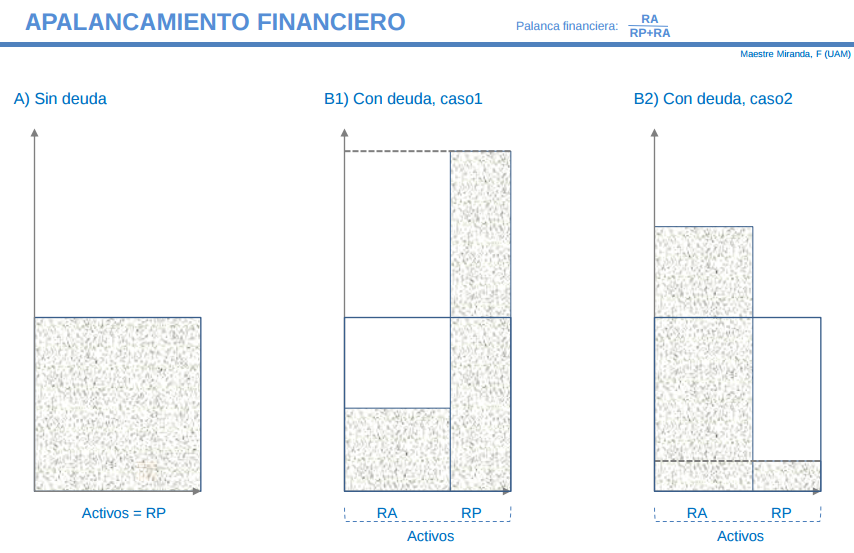
\includegraphics[width=\textwidth]{img/apalancamiento.png}
\caption{Las tres empresas tienen el mismo capital (los mismos recursos) pero con distinta proporcion de RA (Recursos Ajenos) y RP (Recursos Propios)}
\label{fig:ApalancamientoFinanciero}
\end{figure}

Para responder a la pregunta debemos atender a la fórmula que mide la palanca financiera:
\[\text{palanca financiera} = K = \frac{RA}{RP+RA}\]

En general, \textbf{y de forma lógica}, a la empresa le interesa endeudarse (apalancarse) siempre que el rendimiento que vaya a sacarle al préstamo, es decir, el ROI, sea mayor que la cantidad de fondos que es necesario recibir del banco, puesto que esos fondos habrá que devolverlos.

Es decir, nos interesa endeudarnos siempre que
\[K < ROI\]
y no nos interesará endeudarnos en caso contrario.

\subsection{Crowdfunding}

\subsection{Cajón desastre}

% Copiado (mal) de los apuntes de Edu. Es cierto que lo he copiado fatal, pero básicamente es lo que dice Miranda en sus clases.

Letras, tenedor, endoso, deudor. Negociar con sus letras y pagar, antender la letra, endosar = traspasar, atenteder = tener fondos para pagarla. EL último tenedor cobra. La justicia va a por el qeue descontó la letra????  Letras del tesoro, letra de 1000, te adelantan y tienes que pagar. Para descontar letras hay que tener fondos, una persona física no puede descontar una letra. Factoring.

Hipotecas titulizar los derechos propios. Se descuentan las cuoas. Dosificar riesgo. Lehman brothers reparte hipotecas de alto riego. Pablo Iglesias: autónomo, módulos vs contabilidad, sujeto pasivo. Crisis de Lehman brother sotra vez. Préstabmos.

Tipos de préstamos: del crédito: la entidad financiera pone un capital a disposición en una cuenta corriente contra la que puedes cargar talones y pagarés. DPréstamo: la entrega efectiva en su totalidad de un capital a cambio del pago de intereses y del mismo.

Herederos: puedes asumir deudas de tus padres, puedes rechazarlas pero ir ajuioci y te las pueden dar. Dación en pago. ROE del bancho es un 30 y pico el spread de un banco es de un 8-9.

Euribor.  scalping, nyse máquinas de opraciones.

Comisiones por desisitir, subrogar, apertura y cambio de condiciones.

Reunificar dedudas. Para negociar un rp´restamo preguntar por el importe, negociar con el director

Tipos de ineterés 10\% a diez años.

Discusión banca pública vs privada????

PRU: rpéstamo renta universitaria funanciado por ICO. ESTAFA. WTF.

\section{Evaluación de proyectos de inversión}
Con todo lo visto hasta ahora hay poco que añadir en esta sección aparte de las definiciones/explicaciones presentes en el apéndice \ref{sec:ProyectoInversion}.

\section{Mercado y márketing}

Esta sección no ha tenido especial peso en el desarrollo de este curso. Nos hemos limitado a dar algunas pinceladas a algunos conceptos relacionados con el Marketing.

Existen 4 tipos de mercados principalmente:
\begin{itemize}
\item \textbf{Competencia perfecta}. Existen numerosas empresas que pelean en igualdad de condiciones y los precios fluctúan en función de la oferta y la demanda. Todas las empresas compiten por ofrecer lo mejor a sus clientes.

\item \textbf{Competencia monopolística}
Es un tipo de competencia en la que existe una cantidad significativa de productores actuando en el mercado sin que exista un control dominante por parte de ninguno de estos en particular. Ésta es muy frecuente dentro de los mercados de productos que se encuentran normalmente en los supermercados, donde existen productos de diferentes marcas, pero con características particulares y dentro de cada grupo de producto, las características los hacen diferentes unos de otros, pero lo suficientemente parecidos para competir con otros productores y entre sí.
\item \textbf{Oligopolio homogéneo y diferenciado}
Existen muy pocas empresas pero sus productos son muy parecidos entre si.
\item \textbf{Monopolio}
Existe una única empresa que controla todo el mercado, con lo que puede modificar los precios a su antojo sabiendo que los clientes no tienen otra opción.
\end{itemize}

De cara al desarrollo y comercialización de un producto, atendimos a la charla dada por unos compañeros que desarrollaron una aplicación llamada \href{buscarurl}{jamming}.

Uno de los conceptos más importante que pudimos sacar en limpio de esta charla (y que no hayamos mencionado ya a lo largo de estos apuntes) es el concepto de \concept{Producto mínimo viable}. La idea es sencilla: No podemos esperar hasta que el producto está absolutamente completado para sacarlo a la venta pues pueden adelantarse y robarnos la idea y, en caso de salir mal el negocio, habremos invertido demasiado tiempo.

El objetivo de este producto mínimo viable es poder presentar algo a los clientes de forma que podamos empezar a obtener feed back lo antes posible, garanticemos nuestro hueco en el mercado, y podamos centrar nuestros esfuerzos en los aspectos que realmente están funcionando.


\newpage
\section{Apéndice}

\label{sec:CreacionEmpresa}
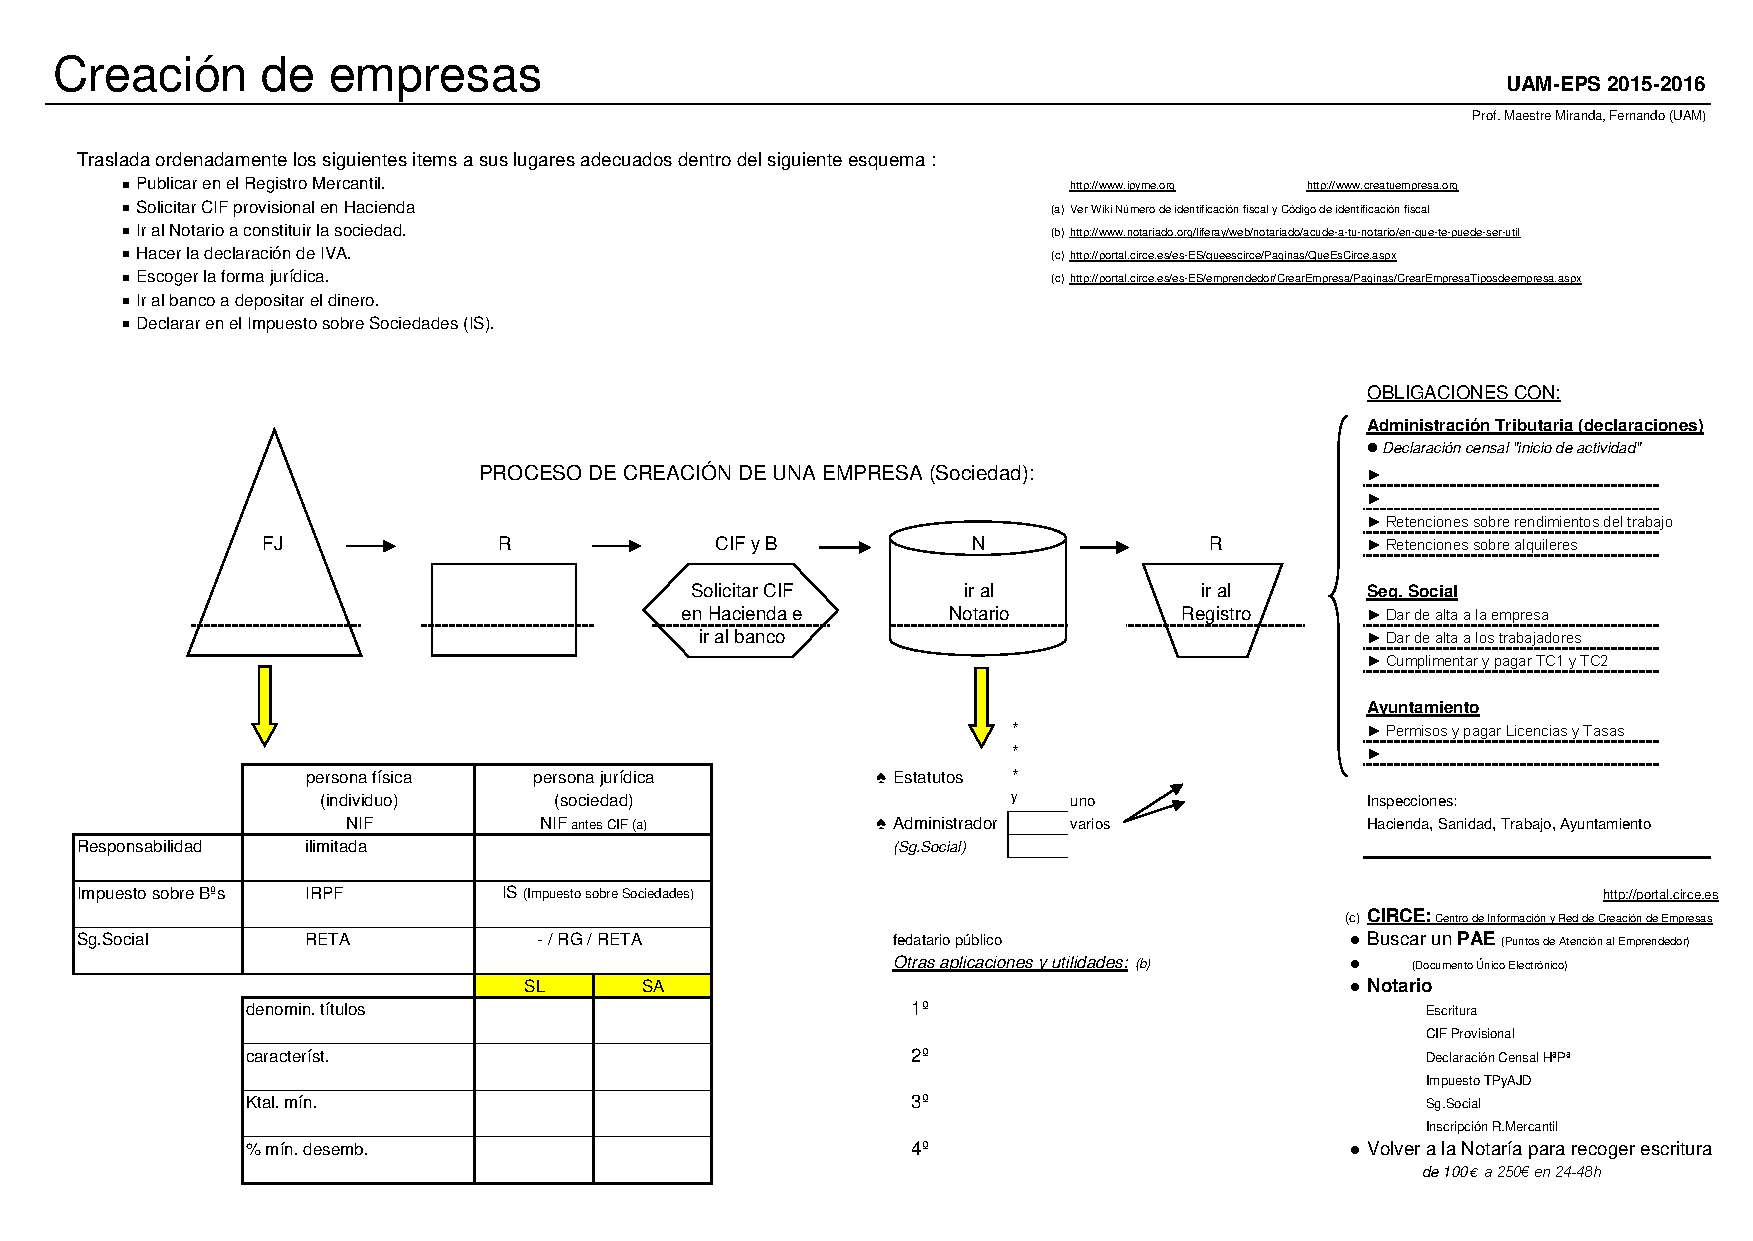
\includepdf[landscape=true, frame=true, noautoscale=true, delta=10 10]{pdf/_creacionEmpresa.pdf}

\label{sec:cicloExplotacion}
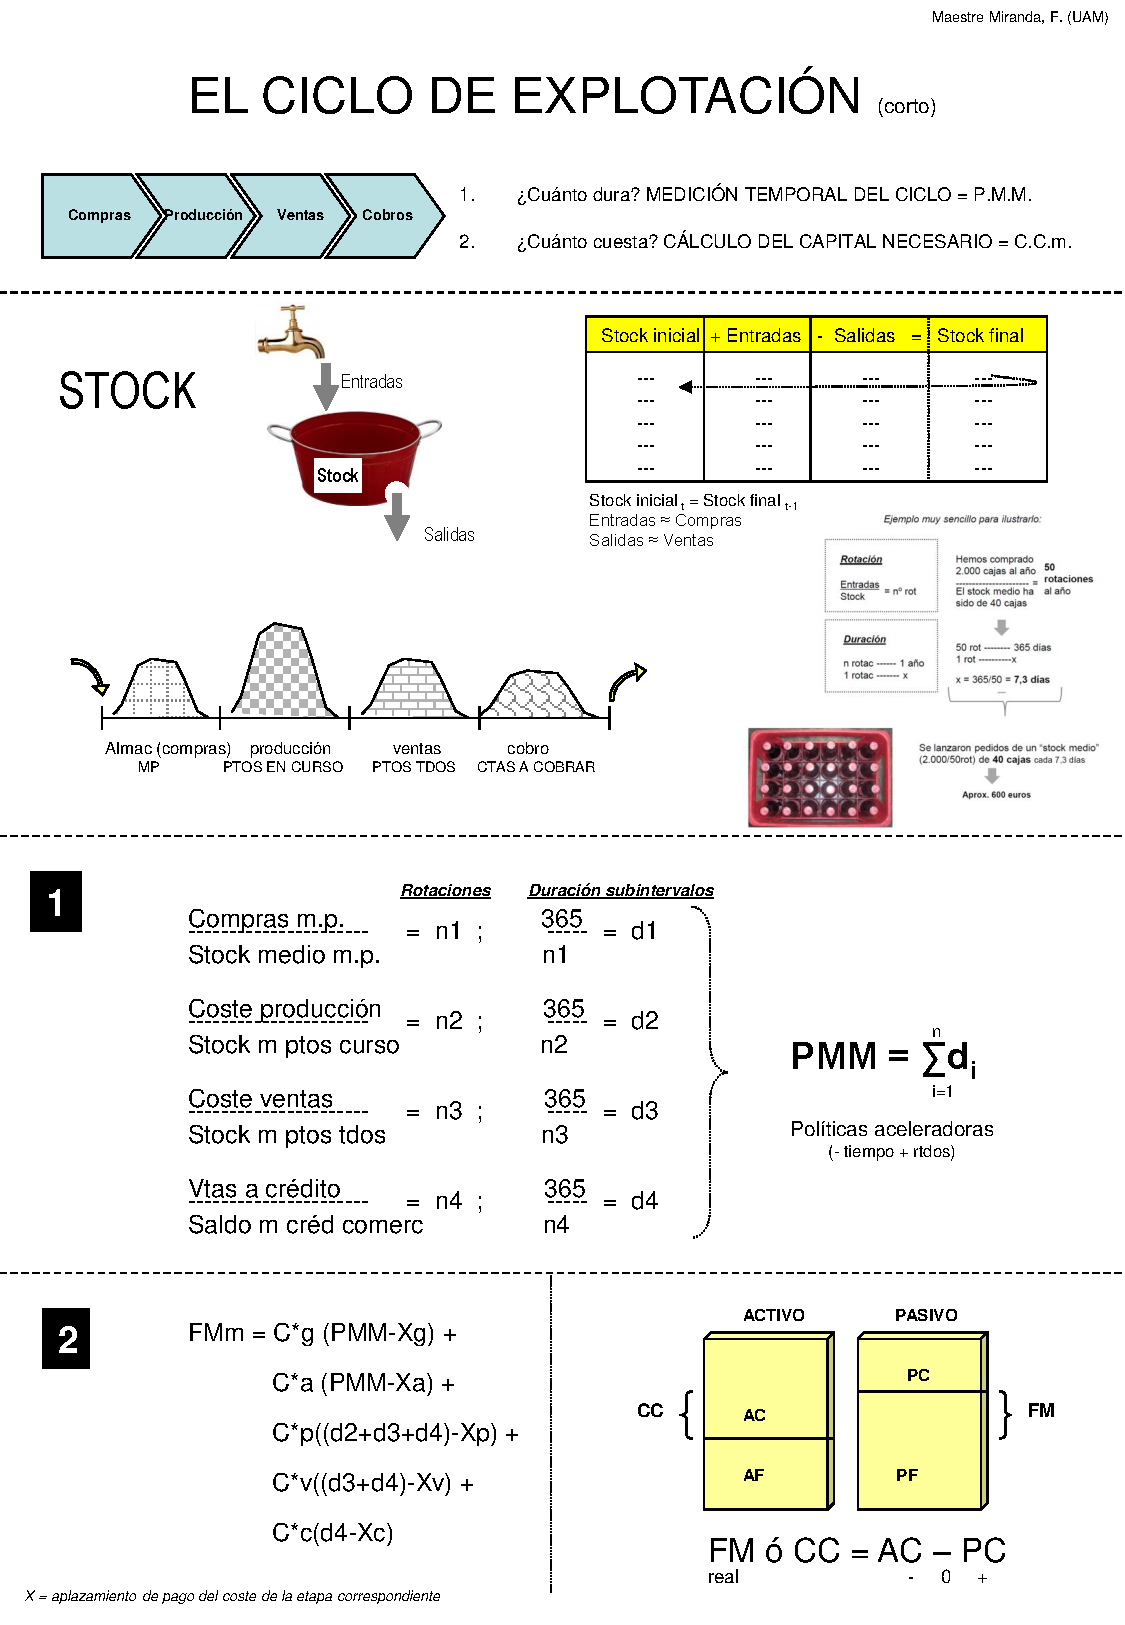
\includepdf[pages={1,2}]{pdf/_Ciclo_explotacion_apuntes.pdf}

\label{sec:contabilidad}
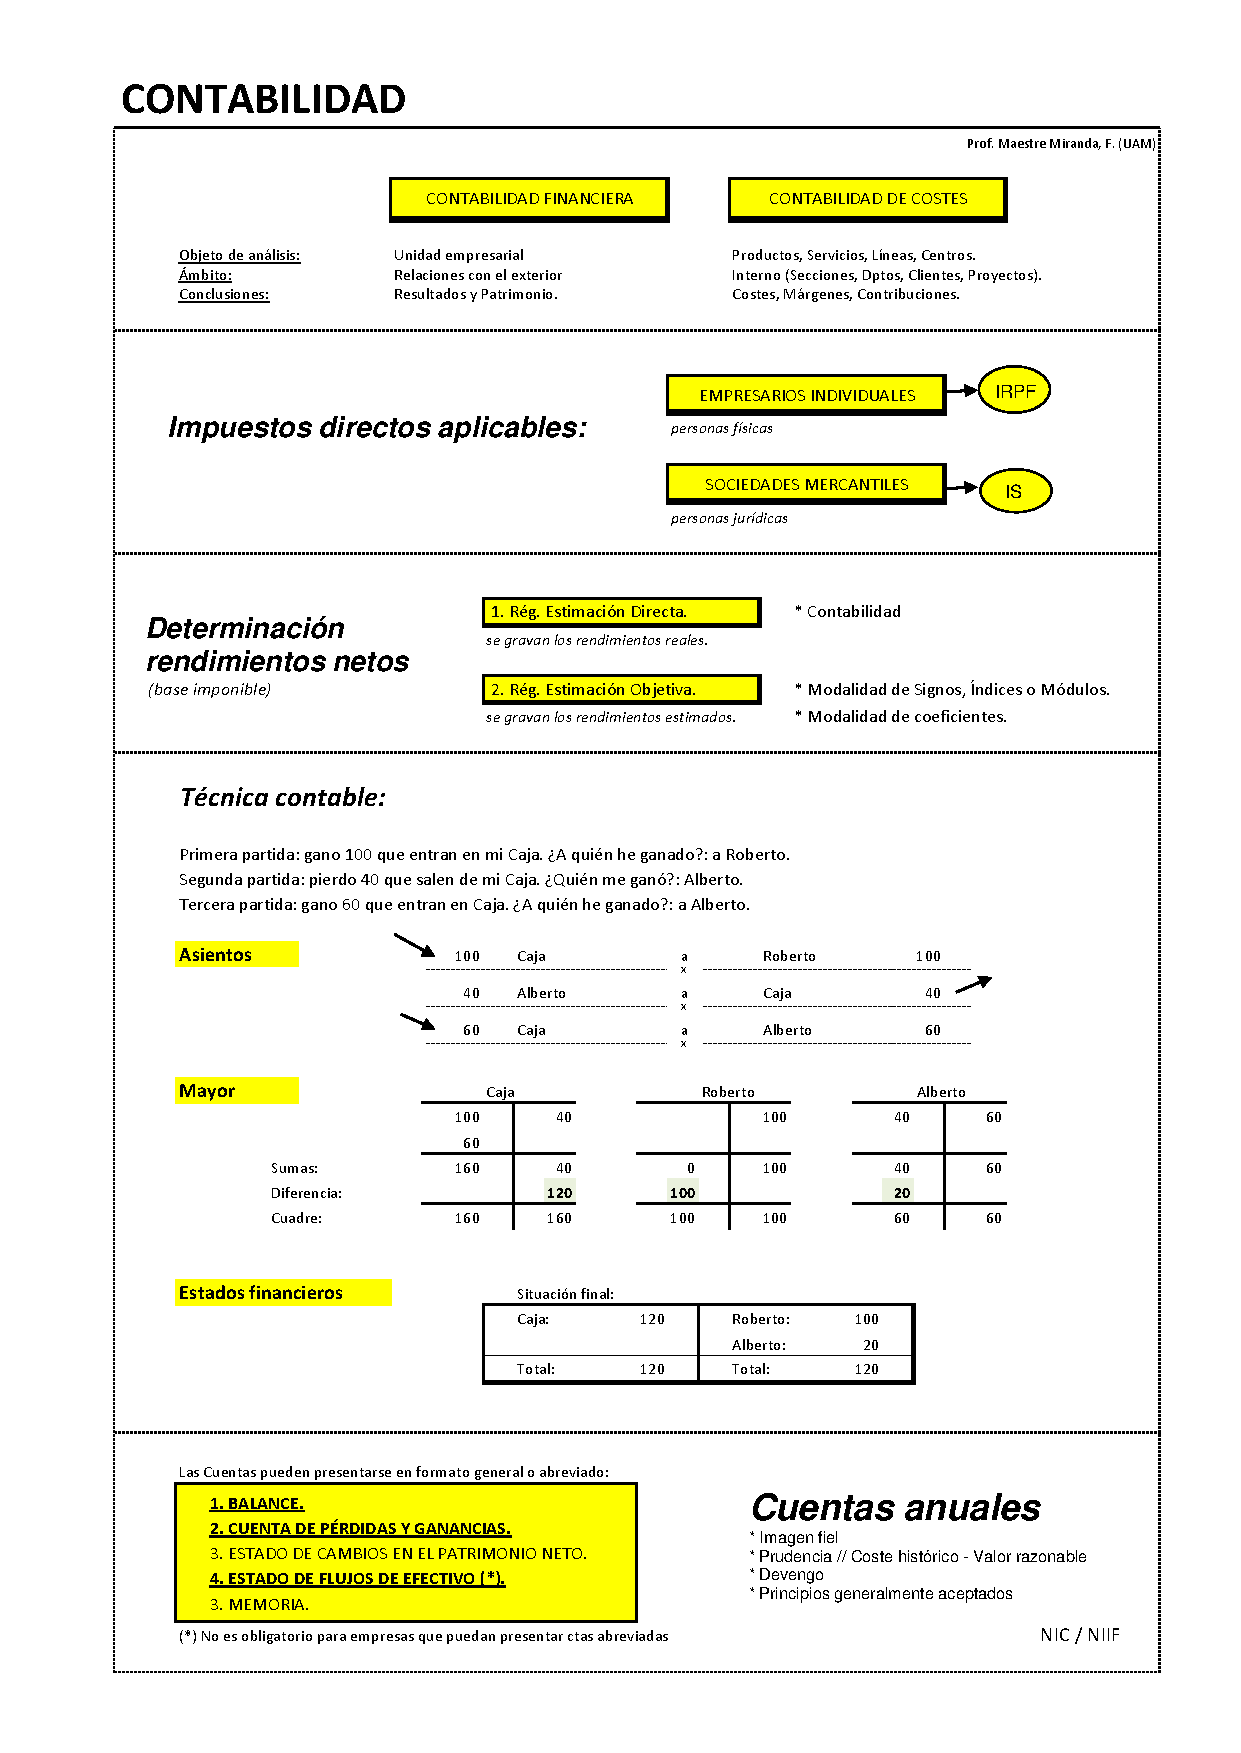
\includepdf{pdf/_Contabilidad.pdf}

\label{sec:circuitoContableIntegrado}
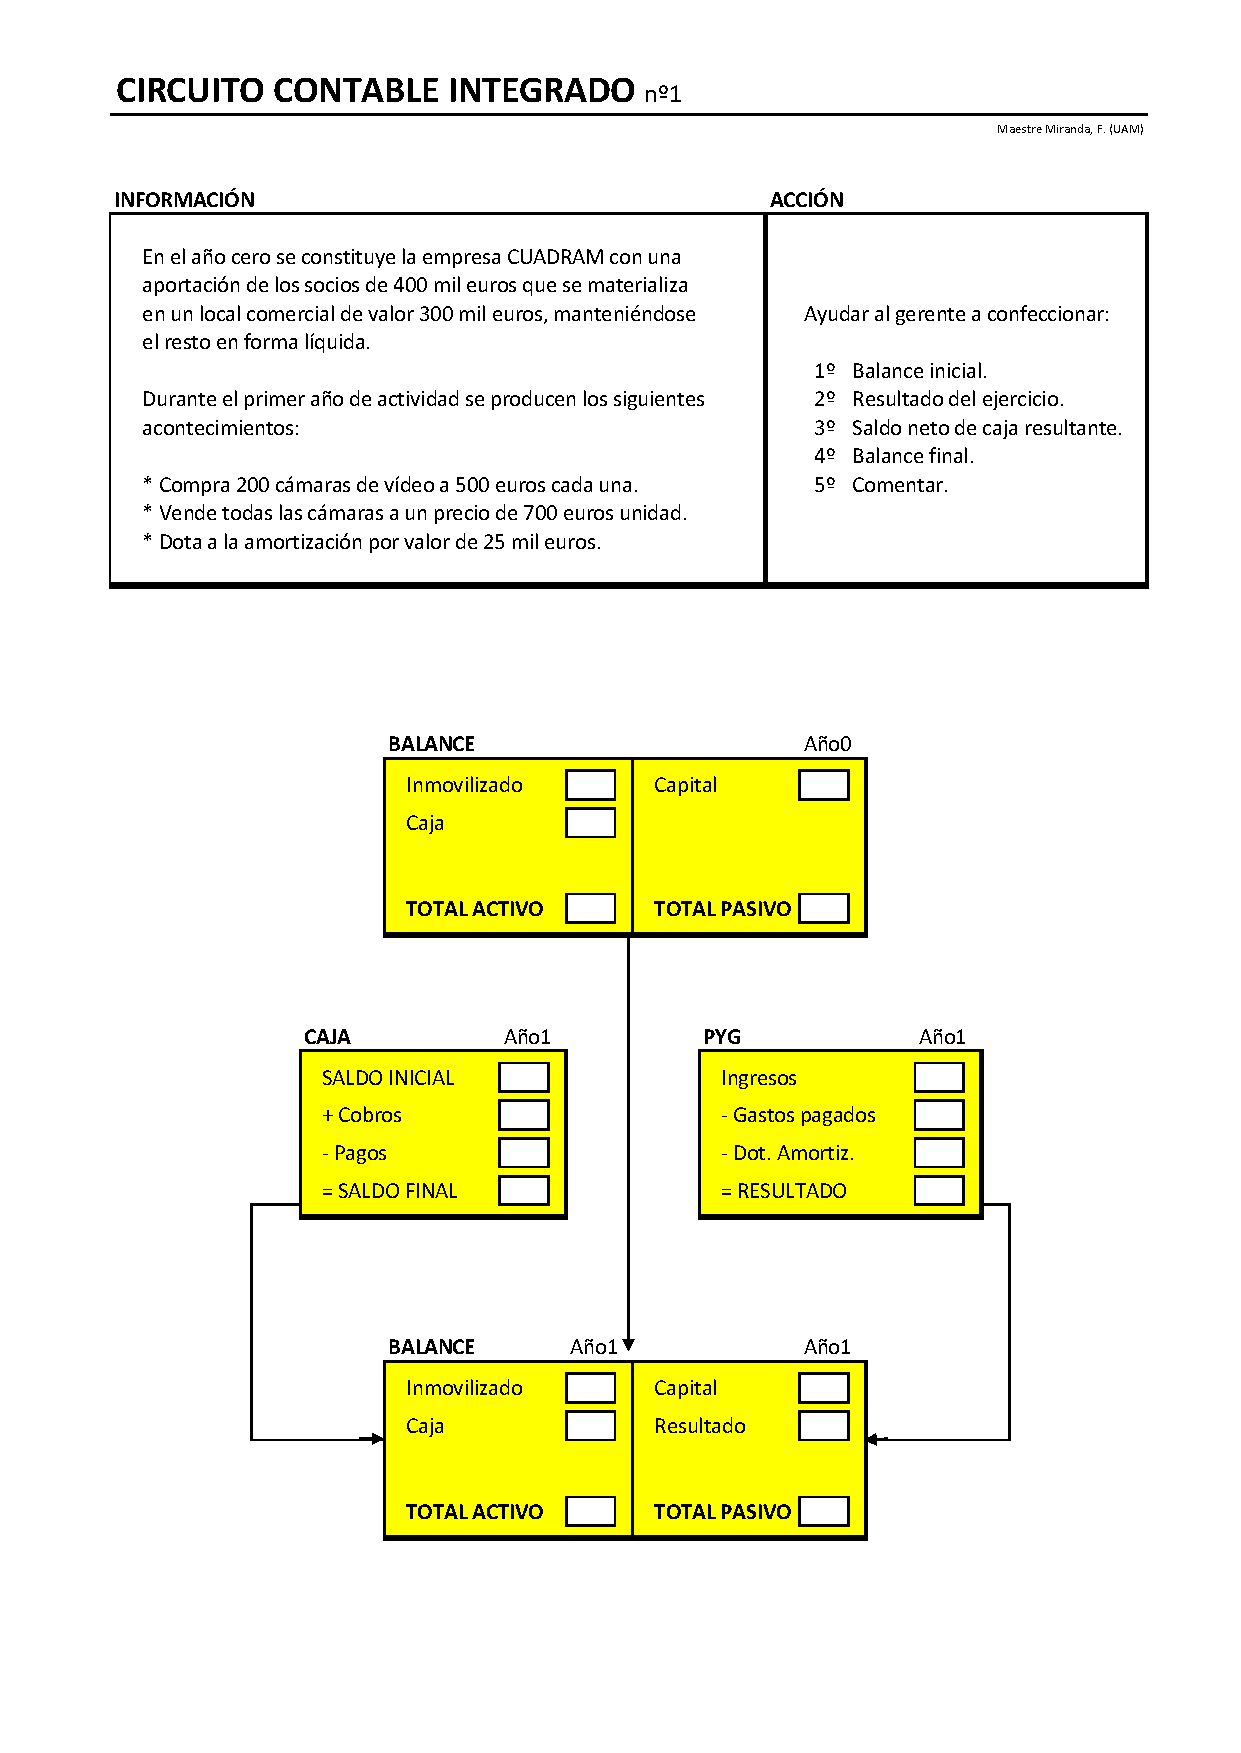
\includepdf{pdf/_CircuitoContable.pdf}

\label{sec:Fruteria}
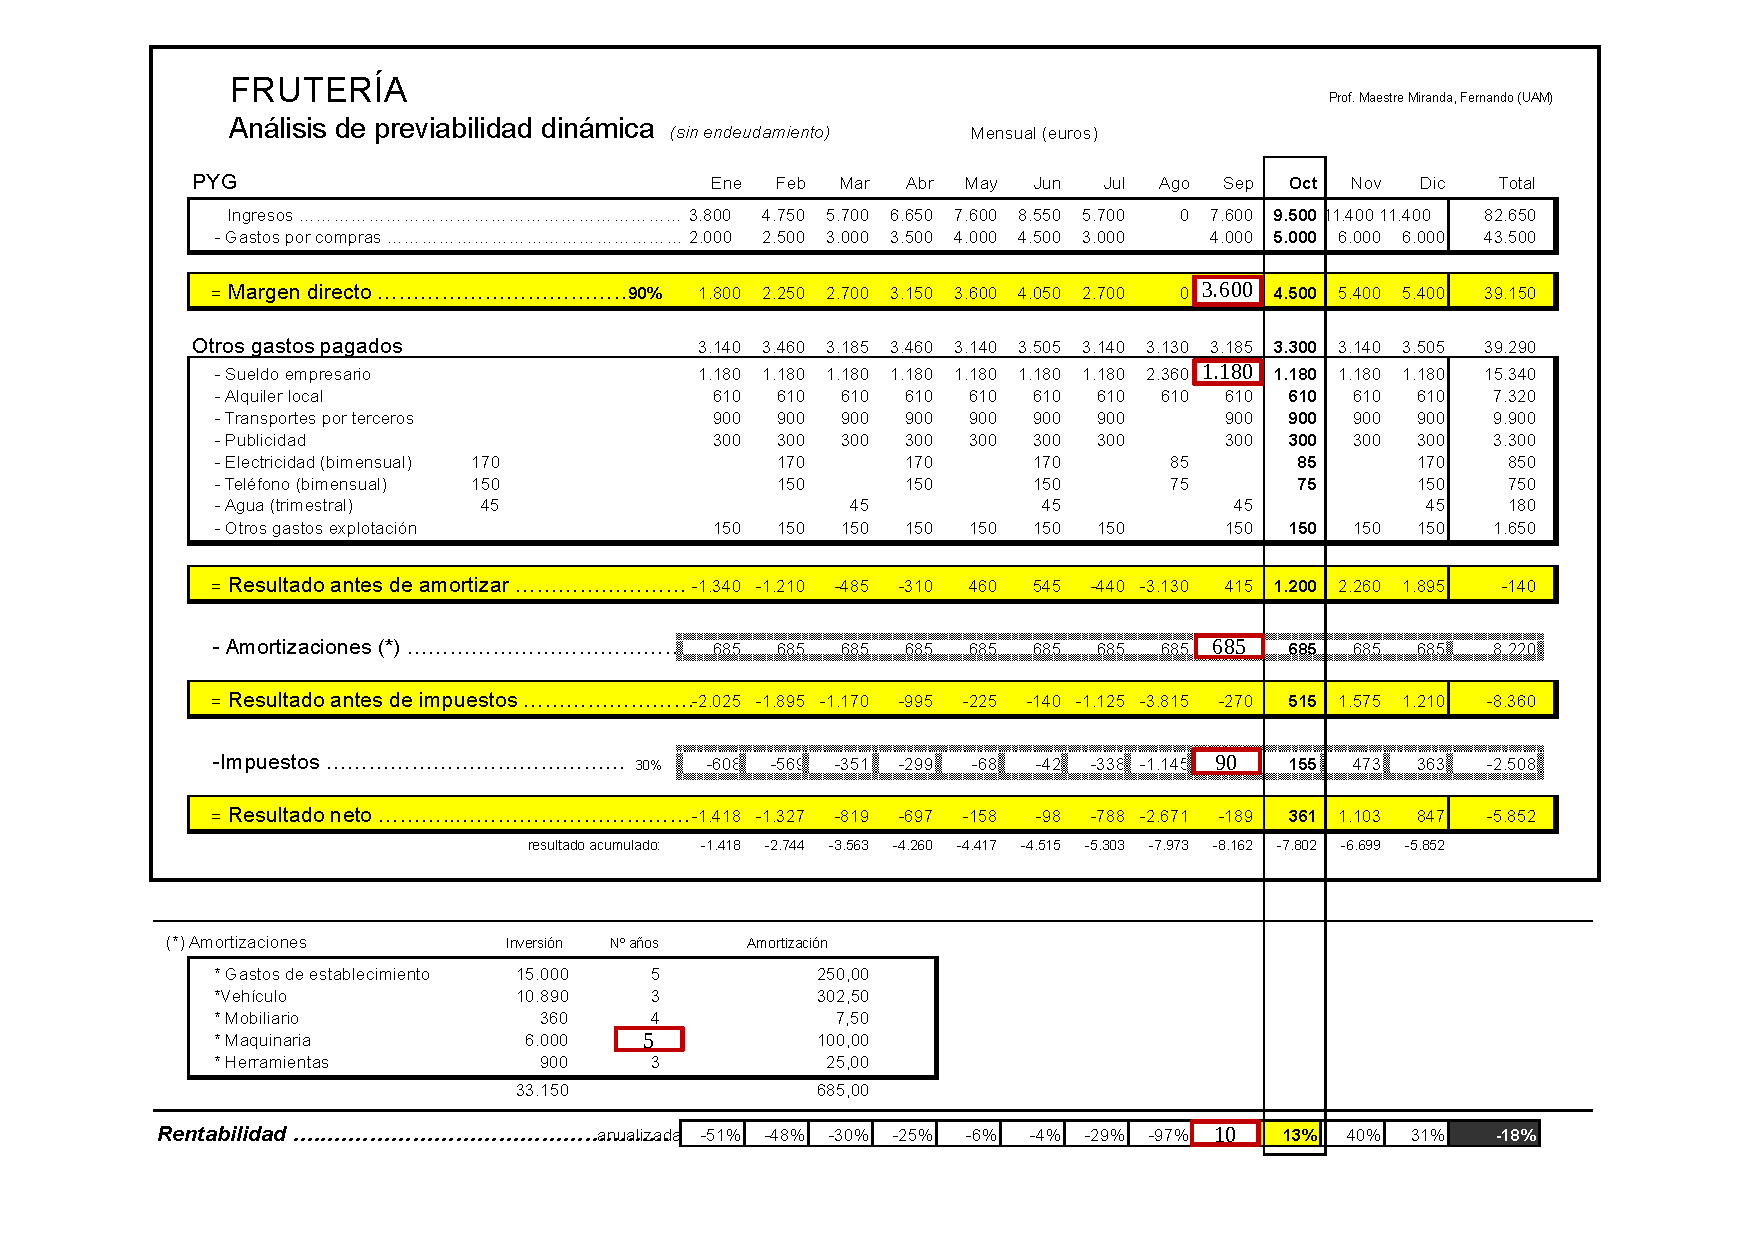
\includepdf[landscape=true, frame=true, noautoscale=true, delta=10 10]{pdf/_Fruteria.pdf}

\label{sec:Prestamos}
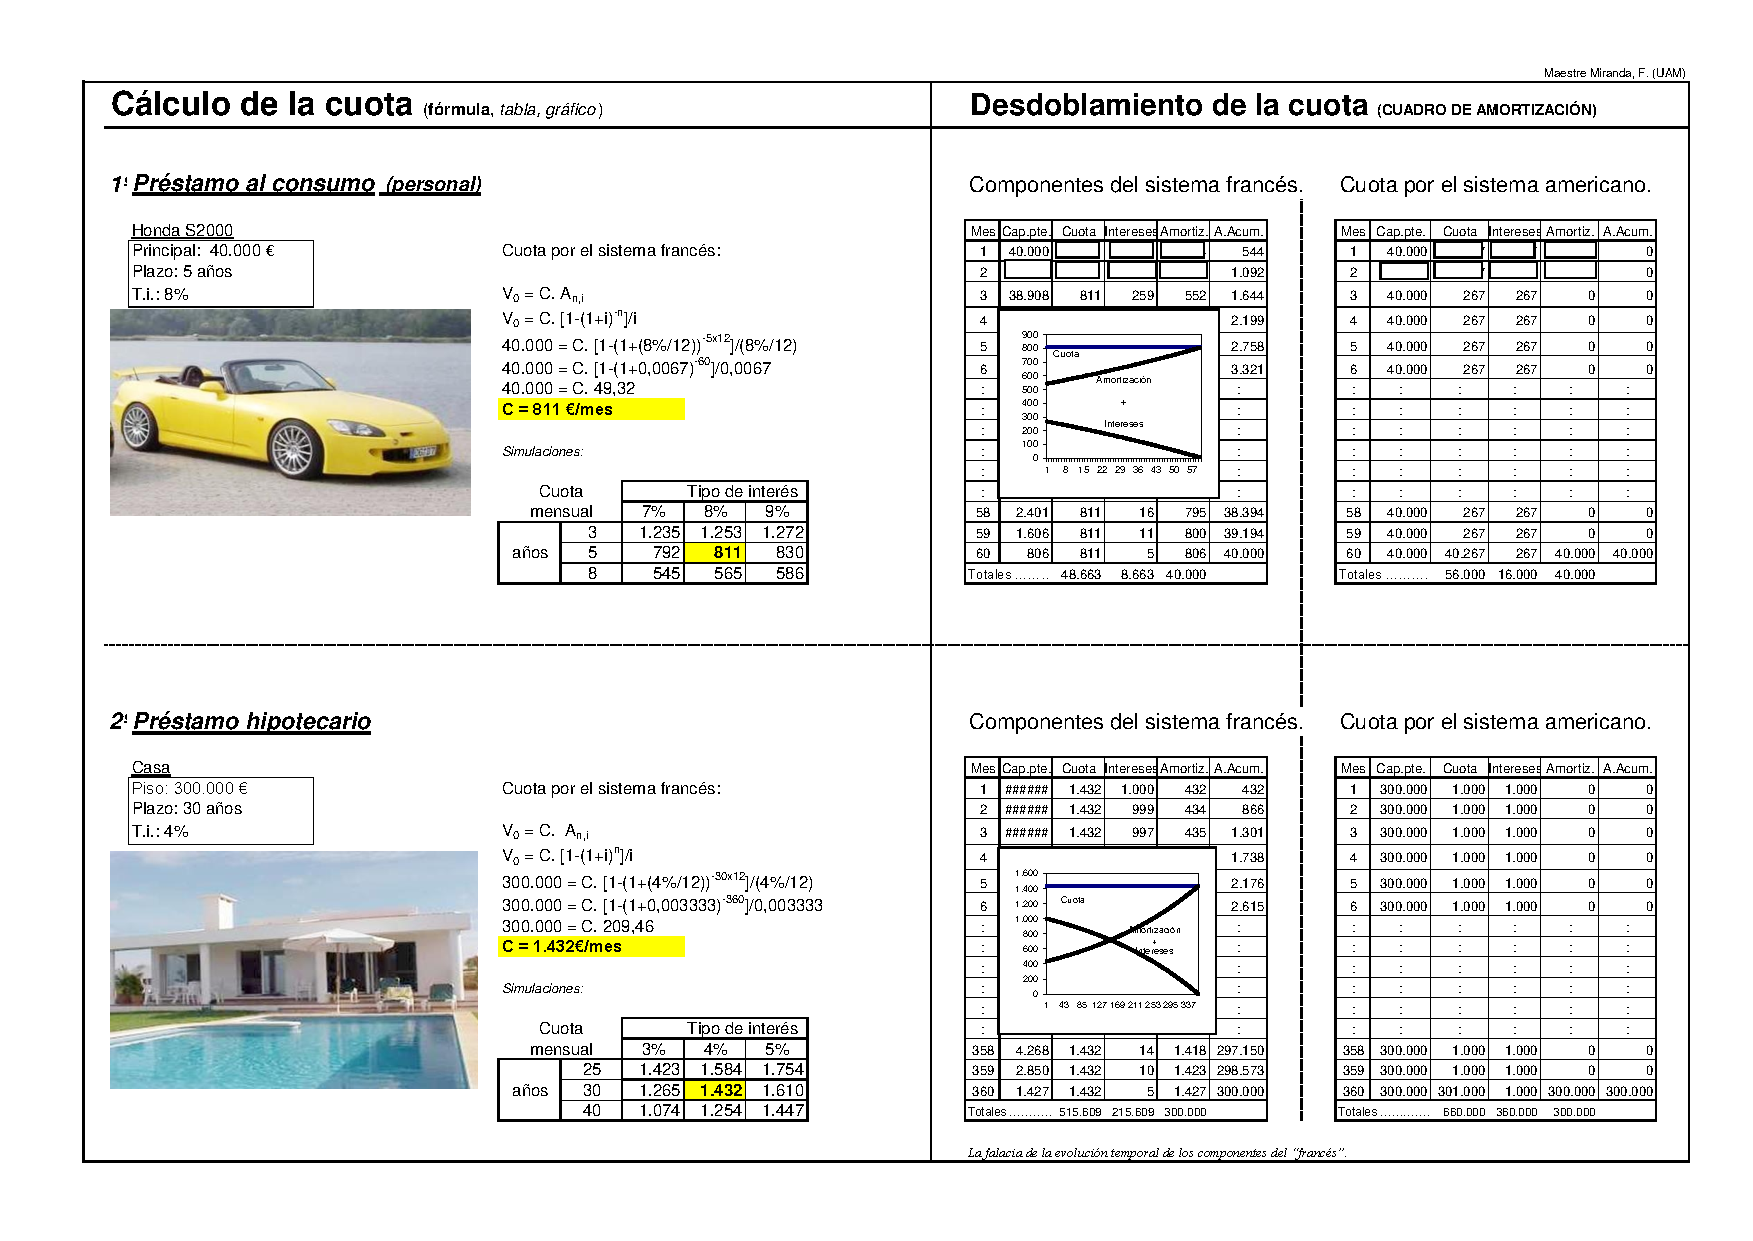
\includepdf[landscape=true, frame=true, noautoscale=true, delta=10 10]{pdf/_Prestamos.pdf}

\label{sec:ProyectoInversion}
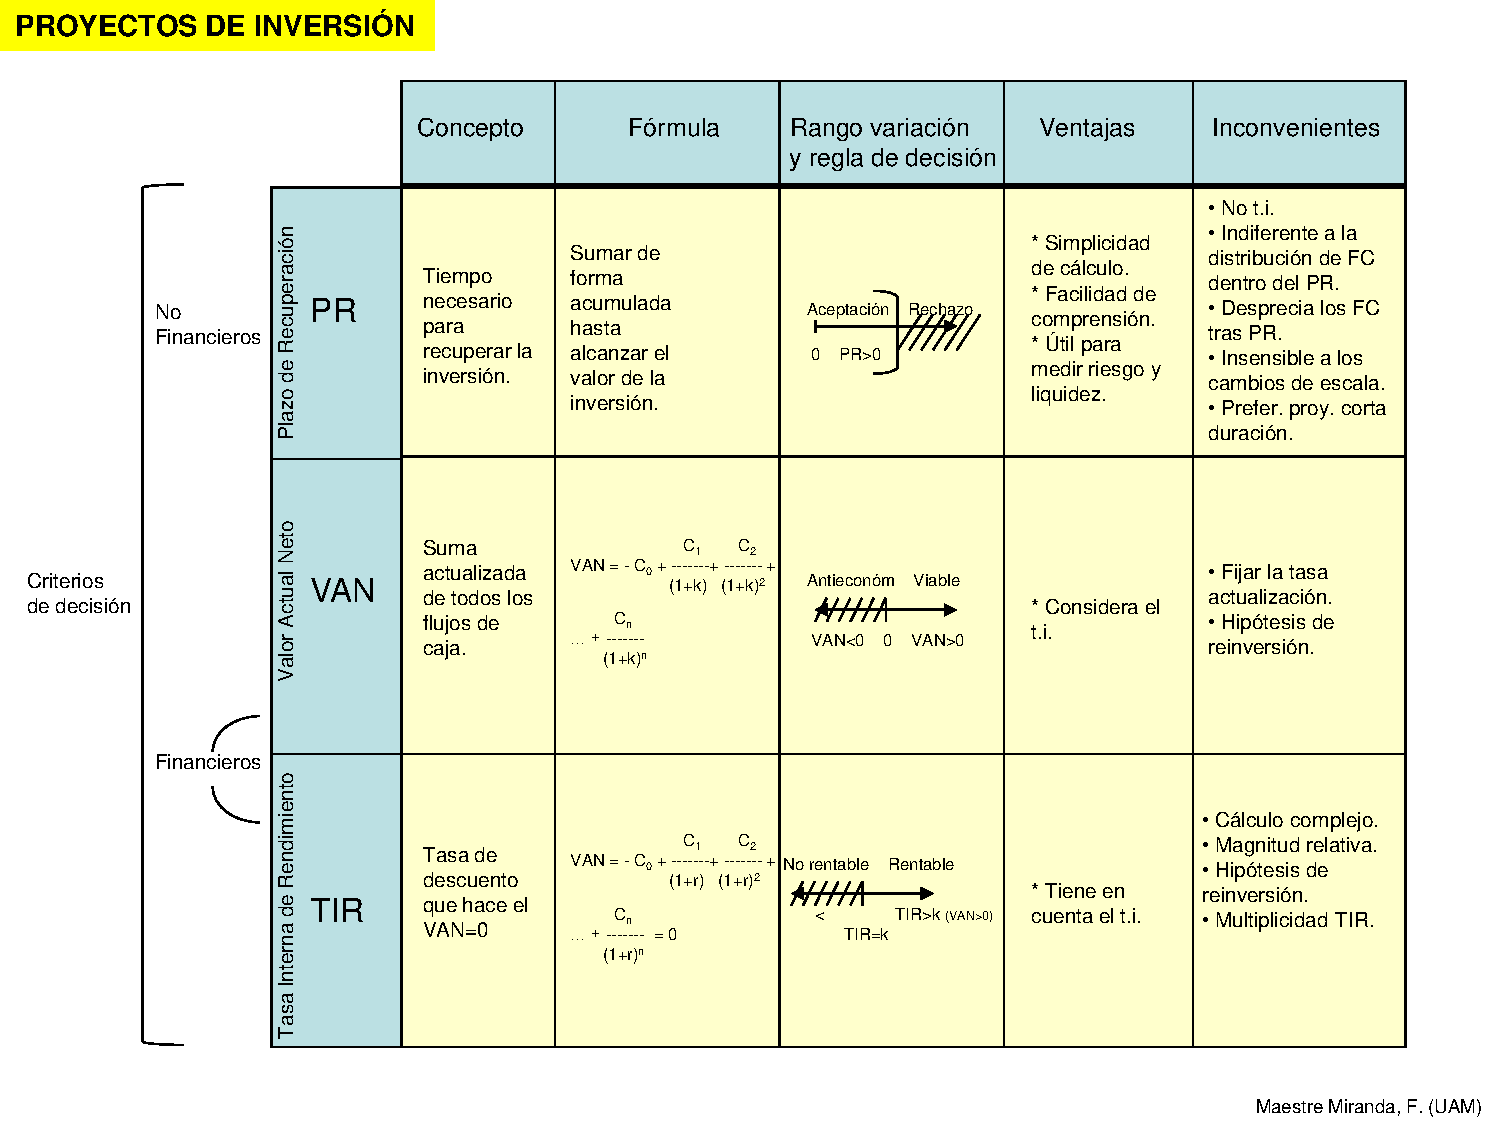
\includepdf[landscape=true, frame=true, noautoscale=true, delta=10 10]{pdf/_ProyectoInversion.pdf}


\printindex
\end{document}
